\section{Eletrônica}
\par A solução de eletrônica do projeto consiste em garantir todo o funcionamento eletrônico do projeto, que é composto pelas áreas: telemetria, sensoriamento e controle do abastecimento e ignição do foguete.
\par Como o principal objetivo do projeto é construir um sistema de controle e monitoramento do foguete que permita isso ser feito a uma distancia segura. Para isso, foi pensada uma solução envolvendo telemetria tanto para colher os dados quanto para enviar sinais de comando. Para melhor detalhamento do projeto na parte de \textit{hardware}, a figura \ref{fig:Diagrama de Blocos} no apêndice \ref{Diagrama de blocos do sistema} resume bem a solução proposta.

Dado os avanços e o melhor desenvolvimento das ideias da proposta de solução da eletrônica, foi construído um diagrama geral mais detalhado, no qual foram incluídos os tipos de protocolos, quantidade de fios necessários e as demais informações que foram pesquisadas no ponto de controle 02. O novo diagrama pode ser visto no seguinte link \href{https://drive.google.com/file/d/12-pXv5L2Z5AuyWWVIr8VZ4WMghu7SYDw/view?usp=sharing}{Diagrama Geral}.     

%%\begin{center}
%%\begin{figure}[H]
%%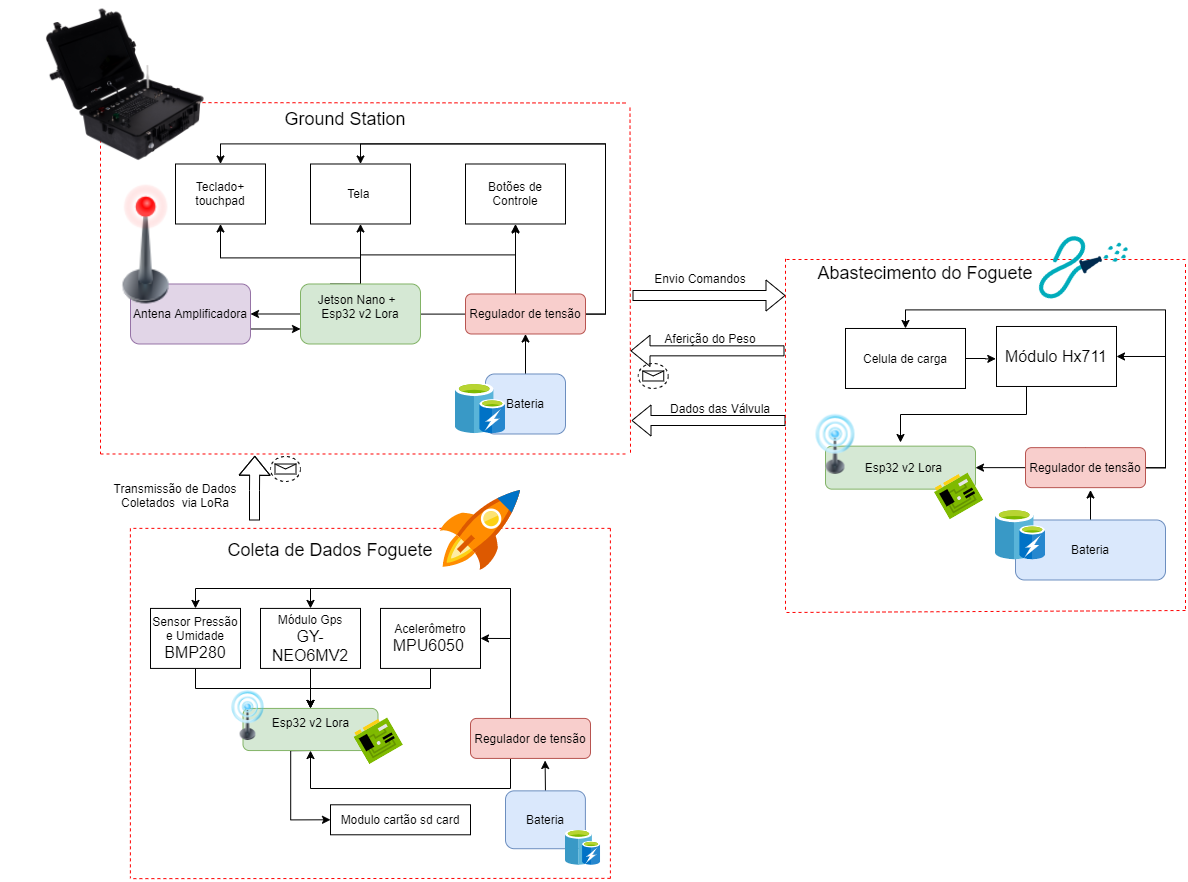
\includegraphics[scale=0.4]{editaveis/solucao/eletronica/diagrama pi2 (2).png}
%%  \caption{Diagrama de blocos do projeto.}
%%  \label{fig:Diagrama de Blocos}
%%\end{figure}
%%\end{center}

\subsection{Telemetria}
\par É um processo remoto de aquisição ou envio de dados, ou seja, é utilizado para medir, rastrear ou até mesmo controlar à distancia alguma coisa. Esse processo é feito geralmente por um sistema de comunicação sem fio, como por exemplo por radiofrequência ou via satélite. \cite{Telemetria_AERONALTICA}.
\par Atualmente,  a telemetria está presente em diversos ramos da vida cotidiana do ser humano: na apuração das informações de um automóvel, no controle meteorológico, na agricultura e em outras diversas atividades.Para o projeto proposto, entende-se que o uso da telemetria em tempo real é extremamente vantajoso para a aquisição de dados durante o voo do foguete e para o controle autônomo do seu abastecimento/ignição.
\par Como requisito de segurança, é necessário fazer o controle  do foguete à distância. O recomendado pelas regras da LASC, competição a qual o cliente pretende participar, é uma distância mínima de 500m (lembrando que o foguete pode atingir uma altura de voo de aproximadamente 1km). Ou seja, fazer a aquisição de dados e o controle de abastecimento e ignição via cabo seria muito dispendioso, ou mesmo inviável, sujeito a maiores riscos de falhas, ou ficando na dependência de coletar os dados armazenados na memória do foguete somente após sua recuperação. Por essas razões, entende-se que é necessário realizar a telemetria em tempo real. Para melhor entendimento, na figura \ref{fig:Diagrama lançamento}   encontra-se o esquemático de um lançamento de foguete.
\begin{figure}[!htb]
\centering
\includegraphics[scale=0.4]{figuras/LANÇAMENTO.png}
\caption{Diagrama do Lançamento.}
{\footnotesize Fonte: Elaborado pelo autor.}
\label{fig:Diagrama lançamento}
\end{figure}

\par Como trata-se de uma função específica, o controle à distância e a aquisição de dados do pré-lançamento, do lançamento, do apogeu até a chegada do foguete no chão, é necessário compreender o problema e levantar requisitos para escolher a melhor forma de fazer a telemetria do projeto.
\par Foram analisadas diversas formas de fazer a telemetria, entre elas estão: a telemetria feita por radiofrequência, Lora, Wi-Fi, ZigBee, GPRS, Bluetooth, entre outras, analisando os seguintes requisitos: 
\begin{itemize}

\item Alcance;
\item Taxa de Transição de dados;
\item Protocolo de Comunicação;
\item Frequência dos Protocolos;
\item Potência de Transmissão; 
\item Interface de Dados;
\item Consumo.

\end{itemize}

\par Por fim, analisando diversos componentes, foi definido que a Placa Lora Esp32 da HELTEC figura \ref{fig:Placa Esp32 Lora } atende os requisitos do projeto citados acima, garantindo assim o funcionamento de qualidade do projeto, sendo que o principal motivo foi a distância alcançada pelo transmissor.

\begin{figure}[!htb]
\centering
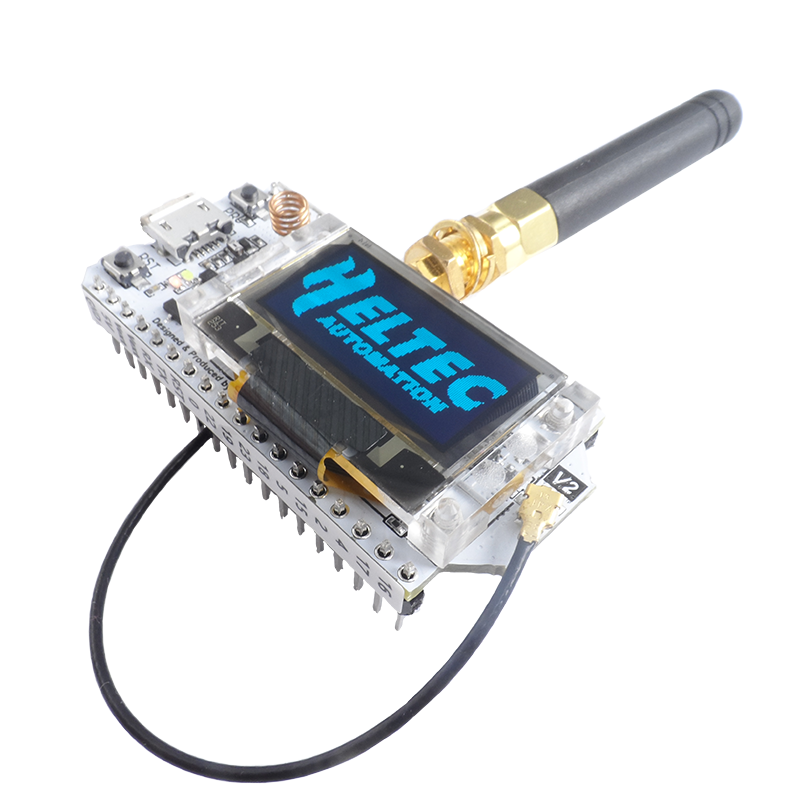
\includegraphics[scale=0.3]{figuras/SAM_0748_800X800.png}  
\caption{Placa Lora Esp32 da HELTEC.}
{\footnotesize Fonte:\cite{datasheet_ESP32}}
\label{fig:Placa Esp32 Lora }
\end{figure}
\par Contudo, como forma de garantir a integridade dos dados, foi pensado em ter um cartão MicroSD para gravação dos dados, evitando assim a perda de dados por falha na telemetria. 


%\par Ainda será feito um levantamento do tamanho do pacote de dados que será gerado por cada sensor, a fim de obter uma análise completa do tamanho da informação que necessitará ser transmitida. Dependendo se a máxima taxa de dados transmitidos por segundo não conseguir suprir o tamanho do pacote gerado será necessário buscar alternativas para superar este problema como por exemplo adotar métodos de codificação\cite{Telemetria_AERONALTICA}. 

\subsubsection{Lora}

\par A comunicação feita via Lora(Long Range) é um método de comunicação à distância sem fio, utilizando radiofrequência e pode ser considerado um marco para o IOT- internet das coisas, possibilitando diversos projetos com sua utilização.
\par A técnica de modulação utilizado pela LoRa é baseada na modulação \textit{Chirp Spread Spectrum} (CSS), que é bastante semelhante à modulação FSK (\textit{Frequency-shift keying}), onde a frequência varia linearmente ao longo do tempo. Contudo, o LoRa tem um ganho de potência maior em relação a modulação FSK, possibilitando assim maior alcance dos sinais.
\par 
A tecnologia LoRa possui uma carga útil de dados que pode varia entre 2 até 255 bytes, dependendo das configurações a serem utilizadas, além de ser possível alcançar até 50 Kbps. Para isso, é necessário  utilizar artifícios de técnicas de canais \cite{transmissaoLoRa}. A LoRa pode ser utilizada em diversas bandas ISM (Industrial Sientific and Medical), que regula as frequências para livre desenvolvimento industrial, sendo que cada país tem seu órgão responsável para distinguir qual faixa pode ser utilizada. Segundo a Resolução n$^{\circ}$ 726, de 05 de maio de 2020, que regulamenta as faixas livres de frequência no Brasil\cite{resolucao726}, a LoRa enquadra-se na faixa de frequência livre no Brasil, que varia de 902 a 928 MHz, entre outras, sendo que a LoRa opera em 915MHz no continente americano (cf. figura \ref{fig:Faixa de Frequência ISM}) .

\begin{figure}[!htb]
\centering
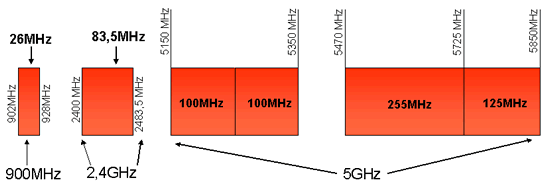
\includegraphics[scale=0.8]{figuras/faixas de frequencia .png}  
\caption{Faixa de Frequência ISM no Brasil.}
{\footnotesize Fonte:\cite{faixafreq}}
\label{fig:Faixa de Frequência ISM} %\url{https://www.teleco.com.br/} }
\end{figure}
\par A modulação LoRa codifica a mensagem em pulsos de \textit{chirps}, sendo que possui alguns parâmetros importantes para o melhor entendimento do funcionamento do mesmo: a largura de banda, a frequência da portadora e a taxa de código\cite{desepenhoLoRa}.

\par A frequência da portadora é definida como a frequência central da informação, que é especificada pela região utilizada pelo equipamento (como citado anteriormente, a frequência é de 915MHz para o continente americano).

\par A largura de banda (BW) define o tamanho da faixa de frequência que a mensagem vai ser transmitida, ou seja a quantidade de informação que irá caber na mensagem. No protocolo de comunicação LoRa, há 3 configurações possíveis programáveis:  125KHz, 250KHz e 500KHz. Já o fator de espalhamento (SF) determina a variação da duração do pulso \textit{chirps} (cf. figura \ref{fig:sflora}), podendo variar de 7 até 12: quanto maior o SF, maior será o tempo da mensagem no ar e, consequentemente, menor o tamanho da mensagem enviada. Na figura \ref{fig:sfloraDISTANCIA}, pode-se notar a representação dessa variante.
\par A taxa de código (CR), por sua vez, é o padrão de correção de erros do LoRa, e é dado pela equação \ref{cr}

\begin{center}
\begin{equation}
\label{cr}
    CR=\frac{4}{4+n}    
\end{equation}
\end{center}
com n variando de 1 a 4 \cite{aplicacaolora}.
\begin{figure}[H]
  \centering
  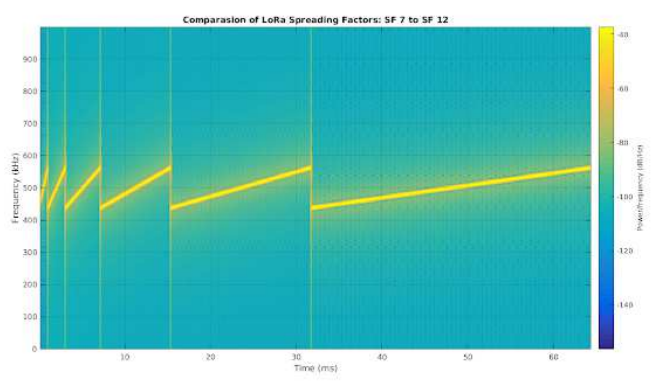
\includegraphics[scale=0.7]{figuras/sflora.png}
  \caption{Diferentes símbolos para SF diferentes em LoRa. }
 { \footnotesize Fonte:\cite{lorasf1}} 
  \label{fig:sflora}
\end{figure}

\begin{figure}[H]
  \centering
  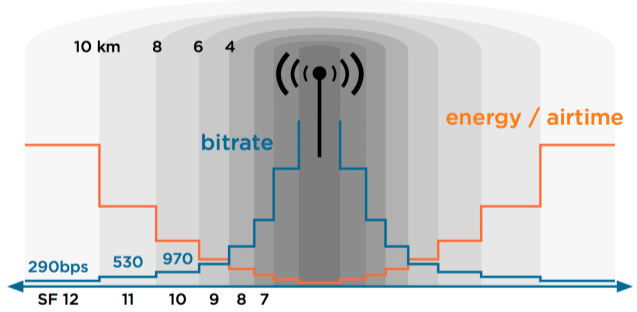
\includegraphics[scale=0.7]{figuras/SFdistanci.png}
  \caption{Diferentes distancias para SF diferentes em LoRa. }
 { \footnotesize Fonte:\cite{lorasf}} 
  \label{fig:sfloraDISTANCIA}
\end{figure}


\par A taxa de bits transmitidas na modulação LoRa pode ser calculada pela equação \ref{taxa de bits }. Na figura \ref{fig:taxalora}, pode-se observar a variação da taxa de transmissão LoRa. Variando o SF e a BW, decidimos usar um SF entre 7 e 8, que atende nossa distancia pretendida com uma largura de banda de 500KHz e uma taxa de código de 4/5 ou 4/6 que garante uma quantidade grande de dados a serem transmitidos.  

\begin{center}
\begin{equation}
 \label{taxa de bits }
 Rb =SF  *  \frac{BW} {2^{SF}}  * CR
 \end{equation}

 \end{center}
Onde:
\par Rb =Taxa de bits/s,
\par BW=Largura de banda,
\par SF=Fator de espalhamento,
\par CR=Taxa de código.


\begin{figure}[H]
  \centering
  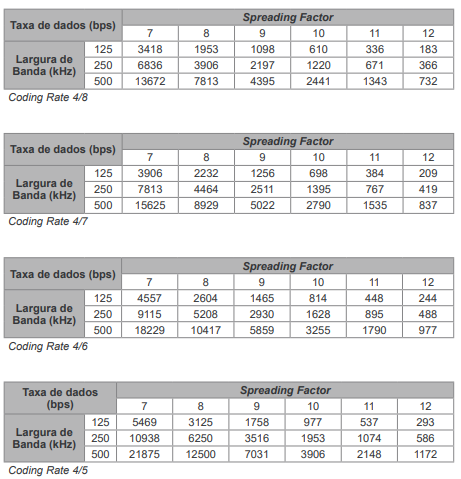
\includegraphics[scale=0.8]{figuras/tabela de taxa lora.png}
  \caption{Diferentes taxa para SF e BW diferentes em LoRa. }
 { \footnotesize Fonte:\cite{aplicacaoloratabela}} 
  \label{fig:taxalora}
\end{figure}


\subsection{Sensoriamento}

Sensores são dispositivos que possuem a função de detectar e responder com eficiência algum estímulo. Existem vários tipos de sensores que respondem a estímulos diferentes, como por exemplo: calor, pressão, movimento, luz e outros. Depois que o sensor recebe o estímulo, a sua função é emitir um sinal que seja capaz de ser convertido e interpretado pelos outros dispositivos \cite{mattede_Sensores_blog2020}.

Definidos os requisitos do projeto, sabe-se que será necessário o uso de sensores e transdutores para a coleta de dados de altitude, velocidade e localização geográfica (GPS) do foguete, e também do peso do foguete durante o abastecimento na sua base de lançamento. Para tal, serão utilizados apenas 3 sensores para obter essas 4 medidas.

\subsubsection{Altitude e Velocidade}

Para medição da altitude e velocidade do foguete durante o lançamento, foi escolhido o sensor de pressão e temperatura BMP280, visto na figura \ref{fig:sensor_pressao} \cite{datasheet_BMP280}.

\begin{figure}[H]
  \centering
  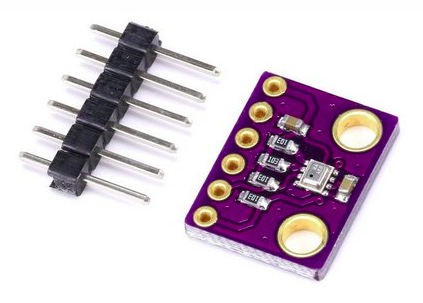
\includegraphics[scale=0.75]{figuras/BMP280.png}
  \caption{Sensor de pressão e temperatura BMP280 (Bosch). }
 { \footnotesize Fonte:\cite{figura_BMP280}} 
  \label{fig:sensor_pressao}
\end{figure}

Esse sensor mostrou-se o mais viável, pois, implementando-o com uso de determinadas bibliotecas, é possível obter os dados de temperatura (Graus Celsius), pressão (hPa) e altitude (metros).

Logo, sabendo a altitude do foguete e obtendo a sua variação ao longo do tempo, este podendo ser medido pelo  \textit{clock} próprio do microcontrolador, é possível medir a velocidade do foguete em cada instante, por meio do cálculo da velocidade média, equação \ref{eq_vel_media}.

\begin{center}
\begin{equation}
\label{eq_vel_media}
V = \frac{\Delta S} {\Delta T}
\end{equation}
\end{center}

onde V é a velocidade média do foguete durante o voo, em m/s, $\Delta$S é a variação de altitude do foguete durante o voo, em metros e $\Delta$T é a variação de tempo de subida do foguete durante o voo, em segundos.

O sensor BMP280 realiza medições de pressão com precisão de $\pm$ 1 hPa e temperatura com precisão de $\pm 1 ^\circ C $. Com essa precisão, é possível realizar medições de altitude com margem de erro de  $\pm$ 1 metro, efetuando a leitura entre 300 e 1100 hPa, o que corresponde à faixa de altitude de +9000 à -500 m \cite{cia_BMP280_2017}.
Em relação aos sensores existentes no mercado, o BMP280 foi o que melhor atendeu aos requisitos, pois ele é a versão mais atual e precisa dos modelos BMP180 e BM085. Também é de baixo consumo em relação aos sensores Mpx10dp e Mpx5700, possuindo melhor aplicabilidade.

Para a implementação do sensor, é necessário o uso de duas bibliotecas da Adafruit para o sensor BMP280 \cite{Adafruit}: a  \href{https://github.com/adafruit/Adafruit_BMP280_Library}{Adafruit\textunderscore Sensor.h} e a \href{https://github.com/adafruit/Adafruit_Sensor}{Adafruit\textunderscore BMP280.h}.

Para ambientes que a Adafruit não pode ser implementada, a Bosh, fabricante do sensor, disponibiliza um código em C para a sua implementação (em \href{https://github.com/BoschSensortec/BME280_driver}{BME280\textunderscore driver}).

As bibliotecas citadas anteriormente já disponibilizam funções, em código C, que retornam as medidas de pressão, temperatura e altitude, tais funções são:

	\begin{itemize}
	    \item float readPressure() -> Leitura da Pressao atmosférica
	    \item float readTemperature() -> Leitura da Temperatura
	    \item float readAltitude -> Leitura da Altitude (em metros, considerando nível do mar)
	\end{itemize} 

Os dados retornados por cada uma dessas funções são do tipo \textit{float}, portanto cada medida tem o dado do tamanho de 4 bytes.

Usando a comunicação I2C, a conexão das pinagens entre o sensor e o microcontrolador foi definida com o SDA e SCL do BMP280 conectados aos pinos D21 e D22 da ESP32 LoRa,respectivamente. Para comunicação, foram conetados o VDD e GND do BMP280 com os pinos 3V3 e GND da ESP32 LoRa respectivamente, conforme mostrado na figura \ref{fig:PINAGEM_BMP280}. 

\begin{figure}[H]
  \centering
  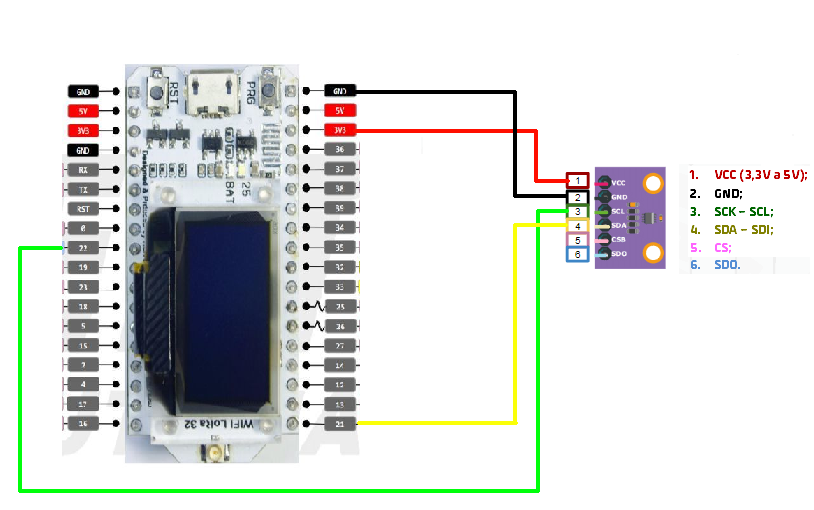
\includegraphics[scale=0.35]{figuras/PINAGEM_BMP280.png}
  \caption{Conexões entre sensor BMP280 e ESP32 LoRa - Protocolo I2C.} 
  {\footnotesize Fonte : Autor } 
  \label{fig:PINAGEM_BMP280}
\end{figure}

\subsubsection{Localização Geográfica (GPS)}

A sigla GPS significa Global Positioning System, o que em português quer dizer Sistema de Posicionamento Global. É uma tecnologia que utiliza satélites e dispositivos para fornecer informações sobre a localização no globo terrestre \cite{fisica_GPS_2020}.
A localização GPS será utilizada para obter a posição geográfica do foguete após sua aterrissagem, podendo também fornecer as coordenadas ao longo do lançamento para determinar a trajetória percorrida pelo foguete.
Foi definido para tal função o GY-NEO6MV2 (Figura \ref{fig:moduloGPS}), um módulo GPS composto por duas partes, a antena, responsável por captar as informações provindas dos satélites e o sistema de controle, responsável pelo processamento dos dados obtidos, por meio do microcontrolador interno NEO6 \cite{datasheet_GPS}.

\begin{figure}[H]
  \centering
  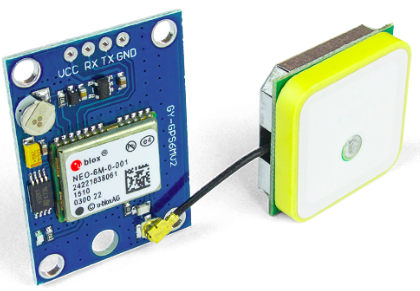
\includegraphics[scale=0.6]{figuras/moduloGPS.png}
  \caption{Módulo GPS GY-NEO6MV2 (uBlox). }
  {\footnotesize Fonte: \cite{figura_GPS}}
  \label{fig:moduloGPS}
\end{figure}

O módulo GPS GY-NEO6MV2 foi escolhido por ser de fácil utilização, realizando a comunicação por meio de comunicação serial, usando apenas 2 pinos (TX e RX), o que permite a comunicação com os mais diversos tipos de equipamentos e microcontroladores. Esse componente apresenta um consumo de corrente em média de 45 mA, enquanto o módulo similar, VK2828U7G5LF, consome em média 50 mA.

Para a aplicação com o módulo é necessário o uso de duas bibliotecas essenciais. A primeira é para a realizar a comunicação serial do microcontrolador com o módulo GPS, onde pode ser usada tanto a biblioteca \href{https://www.arduino.cc/en/Reference/softwareSerial}{SoftwareSerial.h} para usar a IDE do arduino, quanto a biblioteca \href{https://github.com/plerup/espsoftwareserial}{EspSoftwareSerial.h} como exclusivo da ESP32. A segunda (\href{https://github.com/mikalhart/TinyGPS}{TinyGPS.h}) contém todas as funções e comandos necessários para se comunicar com o módulo e acessar suas ferramentas.

Para GPS GY-NEO6MV2, com a vantagem da sua comunicação ser serial, a sua pinagem com a WiFi Lora ESP32 é bastante simples. Portanto, foi definida a conexão dos pinos de VCC e GND do módulo com os pinos 3V3 e GND da ESP32, para alimentação, e conectamos o TX e RX do módulo com os pinos de RX e TX da ESP32 LoRa, usando o procotolo UART de comunicação. A figura \ref{fig:PINAGEM_GPS} mostra as conexões entre os componentes.

\begin{figure}[H]
  \centering
  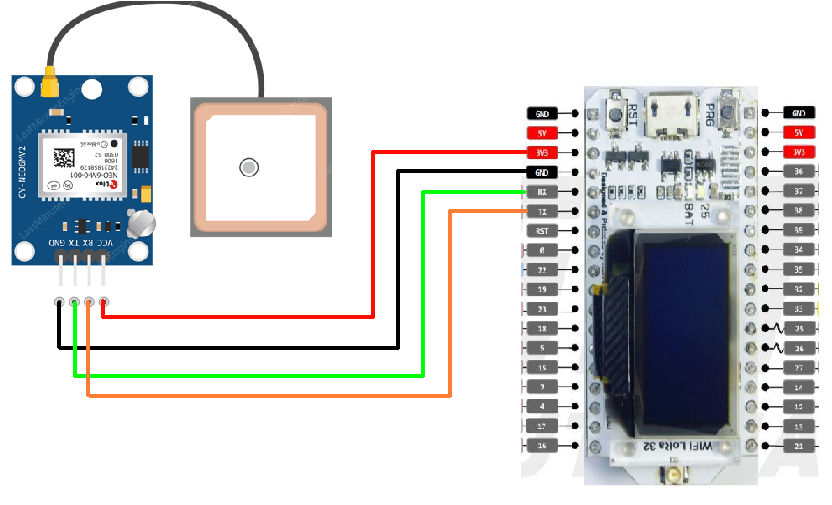
\includegraphics[scale=0.4]{figuras/PINAGEM_GPS.png}
  \caption{Conexões entre o GPS GY-NEO6MV2 e ESP32 LoRa - Protocolo UART.} 
  {\footnotesize Fonte : Autor } 
  \label{fig:PINAGEM_GPS}
\end{figure}


\subsubsection{Peso do foguete}
\label{Peso_do_Foguete}

Por meio do acompanhamento do peso do antes, durante e depois do abastecimento do foguete, será possível controlar e medir a quantidade de combustível contido em seu tanque. Para mensurar o peso do foguete, serão utilizadas duas células de carga. 

Uma célula de carga é um transdutor de força que converte a carga que atua sobre ele em uma saída elétrica mensurável. Embora existam vários tipos, as células de carga baseadas em sensores de deformação e tensão são as mais usadas \cite{omega_celulacarga}. 

Neste projeto, foi escolhida célula de carga de 50 kg (cf. figura \ref{fig:celula_carga}), que atende o peso máximo do foguete, de 18.5 kg com o tanque de combustível cheio e 14.3 kg vazio (dados fornecidos pela Capital Rocket Team).

\begin{figure}[H]
  \centering
  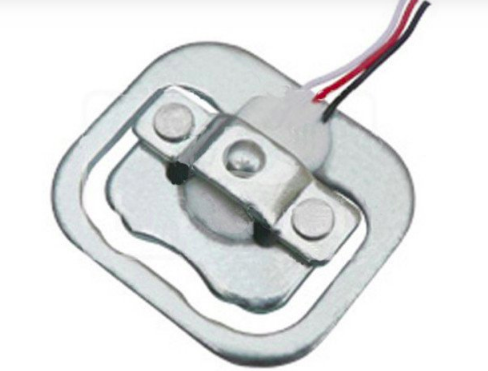
\includegraphics[scale=0.75]{figuras/celula_carga.png}
  \caption{Célula de carga - 50 kg.}
  {\footnotesize Fonte: \cite{figura_celula}} 
  \label{fig:celula_carga}
\end{figure}

Esse é um sensor de carga de meia-ponte da Weadstone, amplamente utilizado em balanças. Quando a meia-ponte é esticada, é enviado um sinal elétrico através de um fio. Utilizando-se apenas uma célula de carga seriam necessários mais resistores para completar a ponte. Além disso, projetos com apenas uma célula de carga tendem a ter dificuldades para ajustes de calibração da célula.

Portanto, considerando também que, além do foguete acima da balança, haverá toda uma estrutura para comportar a base do foguete, serão usadas duas células de cargas para fazer a balança, o que é o mais indicado: uma para medir compressão e outra para medir tensão (forças aplicadas em direções diferentes). Com duas células de carga, tem-se uma ponte de Wheatstone completa.

Como o sinal enviado pelo transdutor é elétrico, precisa-se de um módulo conversor, que fará a conversão do sinal elétrico em sinal digital para possibilitar a leitura dos dados pelo microcontrolador. Para isso, será usado o módulo conversor HX711, figura \ref{fig:conversorHX711}, um módulo amplificador e conversor HX711 de 24 bits, utilizado para amplificar o sinal de dispositivos como células de carga, fazendo a interligação entre essas células e o microcontrolador, por meio da comunicação SPI \cite{avia_HX711}.

\begin{figure}[H]
  \centering
  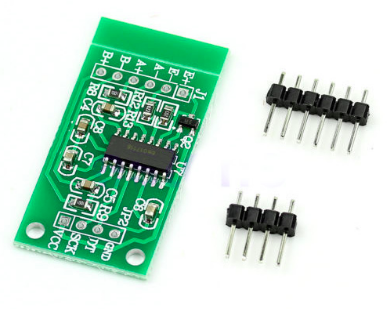
\includegraphics[scale=0.6]{figuras/conversorHX711.png}
  \caption{Célula de carga - 50 kg.}
  {\footnotesize Fonte: \cite{figura_HX711}} 
  \label{fig:conversorHX711}
\end{figure}

Para implementar a balança, a comunicação é feita apenas do microcontrolador com o módulo e amplificador HX711. Para tal, foi definido o protocolo de comunicação I2C, sendo necessário o uso da biblioteca \href{https://github.com/bogde/HX711}{HX711.h}. Nessa biblioteca, a função a ser utilizada,  que retorna os dados do peso da balança é do tipo \textit{long}, ou seja, uma dado de 4 bytes.

As conexões entre o conversor e microcontrolador foram definidas da seguinte forma: para alimentação, o VDD e GND do HX711 conectados nos pinos 5V e GND da ESP32 Lora, respectivamente, para comunicação I2C, o DT e SCK do HX711 conectados nos pinos D23 e D17 da ESP32 LoRa. A figura \ref{fig:PINAGEM_balanca} mostra as pinagens realizadas.  

\begin{figure}[H]
  \centering
  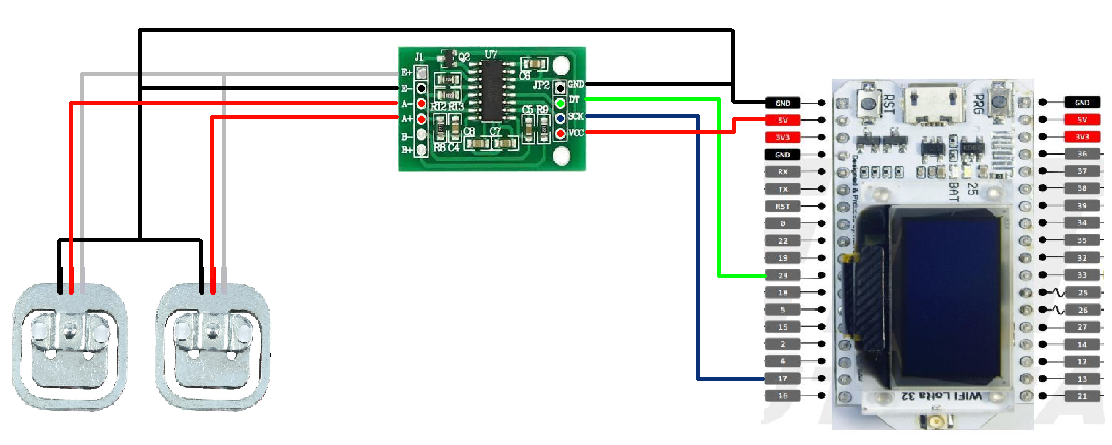
\includegraphics[scale=0.4]{figuras/PINAGEM_BALANCA.png}
  \caption{Conexões entre Hx711 e ESP32 LoRa - Protocolo I2C.} 
  {\footnotesize Fonte : Autor } 
  \label{fig:PINAGEM_balanca}
\end{figure}

\subsubsection{Especificações dos sensores}
A tabela \ref{tab:sensores} apresenta os dados das principais especificações dos sensores citados acima.

\begin{center}
\begin{table}[H]
\centering
\begin{tabular}{ |m{2cm}|m{2cm}|m{2.5cm}|m{2.5cm}|m{2.5cm}|m{2.5cm}| } 
\hline

\textbf{ Sensor }&\begin{center}
\textbf{ Tensão de Operação} \end{center}& \textbf{Consumo de corrente }& \textbf{Comunicação} & \begin{center}\textbf{Taxa de transmissão} \end{center} & \begin{center}\textbf{Formato dos Dados}\end{center}\\ 
 \hline
 
 BMP280 & 1.71 - 3.6V & 3.6 $\micro$uA @ 1 Hz (umidade, pressão e temperatura) & 
I2C e SPI & I2C (até 3.4 MHz e SPI (3 e 4 fios, até 10 MHz) & unsigned 20-bit (pressão e temperatura) unsigned 16-bit (umidade)\\
  \hline
Célula de carga 50kg & 5 -10V & Resistência de entrada e saída ($\ohm$): 1000 ± 50 & - & - & - \\
  \hline
 Módulo Hx711 & 4.8 - 5.5V & 1.5mA & SPI & 10 - 80 MHz & 24 bits em complemento de 2 \\ 
  \hline
 Módulo GPS GY-NEO6MV2 & 3 - 5V & 10mA – 100 mA & Serial UART e SPI & 9600 bps (UART baud rate) e 100 kbit/s & - \\ 
 \hline 

\end{tabular}
\caption{Especificações principais dos componentes do sensoriamento.}
\label{tab:sensores}
\end{table}
\end{center}

\newpage
\subsection{Central de controle}

A central de controle será o ponto de acesso do usuário com os dados e comandos vindos da base de lançamento e do foguete. Um exemplo de estação pode ser visto na figura \ref{fig:DroneStation}. 

\begin{figure}[H]
  \centering
  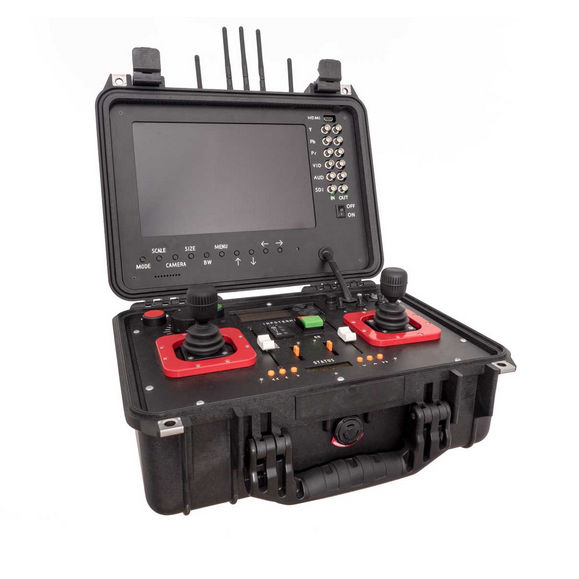
\includegraphics[scale=0.9]{figuras/DroneGroundStation.jpg}
  \caption{Estação de controle de solo.}
  {\footnotesize Fonte : \cite{AeroExpo}} 
  \label{fig:DroneStation}
\end{figure}


A solução proposta para essa interface do usuário foi seguindo esse modelo de maleta, que possui uma tela, um teclado e dois botões, sendo o primeiro para acionamento da ignição e um segundo para interromper os processos em caso de emergência.

\subsubsection{Interface do usuário}

A tela escolhida pode ser vista na figura \ref{fig:Tela}. Essa tela possui um tamanho de 9 polegadas e uma resolução máxima de 1600x1200. 


\begin{figure}[H]
  \centering
  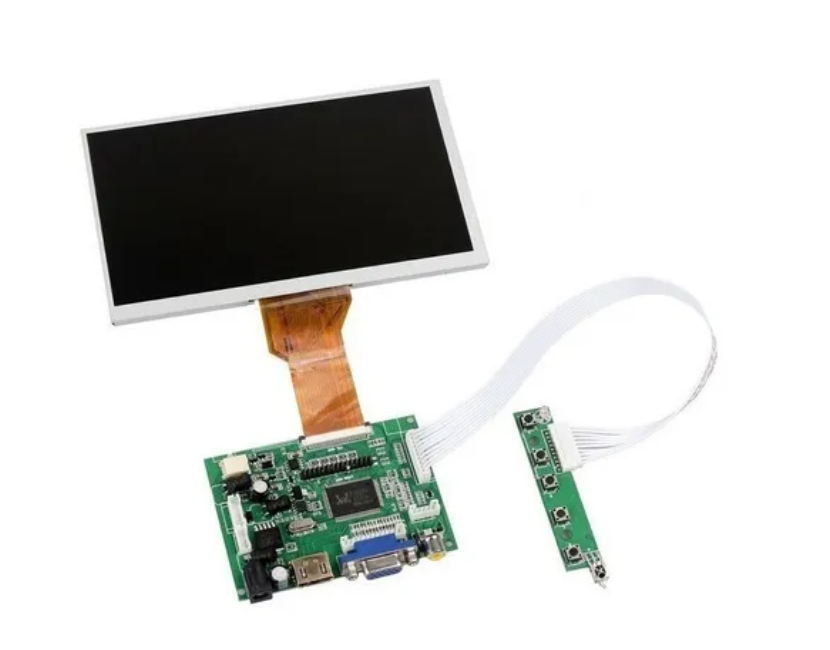
\includegraphics[scale=0.7]{figuras/TELAPI2.png}
  \caption{Tela da interface do usuário. }
  {\footnotesize Fonte : \cite{figura_Tela} } 
  \label{fig:Tela}
\end{figure}

Para a chegada dessa definição, pesquisas foram feitas e percebeu-se que geralmente telas menores, cinco e sete polegadas, possuem sensibilidade ao toque o que além de não agregar mais valor em nosso produto, dificultaria no dimensionamento da bateria dado a maior necessidade de potencia desse tipo de tela. Outro ponto levado em consideração é a questão da troca que existe entre o tamanho da tela e seu gasto energético. Precisava-se de uma tela grande o suficiente para a boa visualização dos dados, porém que fosse portátil e que consumisse pouca carga da bateria. Assim a escolha da tela com as características mencionadas anteriormente é justificada.

Para que o usuário interaja com essa tela, foi pensado em dois tipos de soluções. A primeira seria colocar todos os comandos em botões e chaves, e a segunda realizar os comandos por meio de um mini teclado. Optou-se pelo o uso do teclado, devido a possibilidade de maior interatividade com a aplicação de \textit{software} e facilidade para futuras atualizações no projeto. 

O modelo de teclado portátil escolhido pode ser visto na figura  \ref{fig:Teclado}. Esse teclado possui dimensões de 200x126x6,2 mm e um peso de 200g.

Porém, em conversa com os nossos  \textit{stakeholders}, chegou-se à conclusão que um botão para a ignição e um botão em caso de falha seriam necessários, devido a possibilidade de acontecimento de falhas no processo de lançamento. Assim, esses dois botões também serão integrados à nossa solução.




\begin{figure}[H]
  \centering
  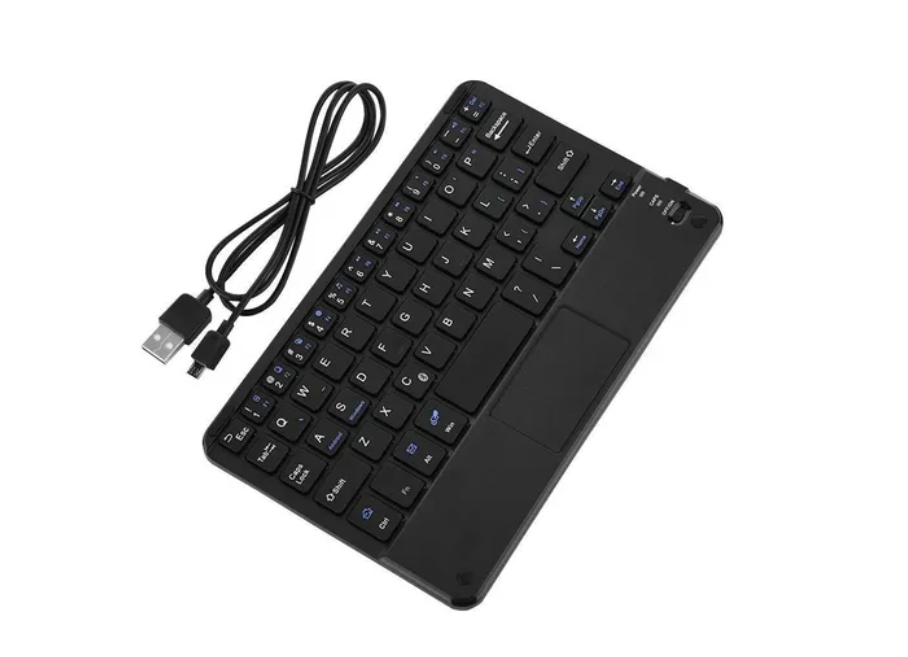
\includegraphics[scale=0.5]{figuras/TecladoPI2.png}
  \caption{Teclado da interface do usuário.}
  {\footnotesize Fonte : \cite{figura_Teclado}} 
  \label{fig:Teclado}
\end{figure}

\subsubsection{ \textit{Single Board Computer}}

Para a melhor escolha da placa utilizada no projeto, foi montada a seguinte tabela, na figura \ref{fig:comparacaoMicro}. Essa tabela foi levada aos grupos de \textit{software} e de energia para o debate entre capacidade de processamento e custo energético.

\begin{figure}[H]
  \centering
  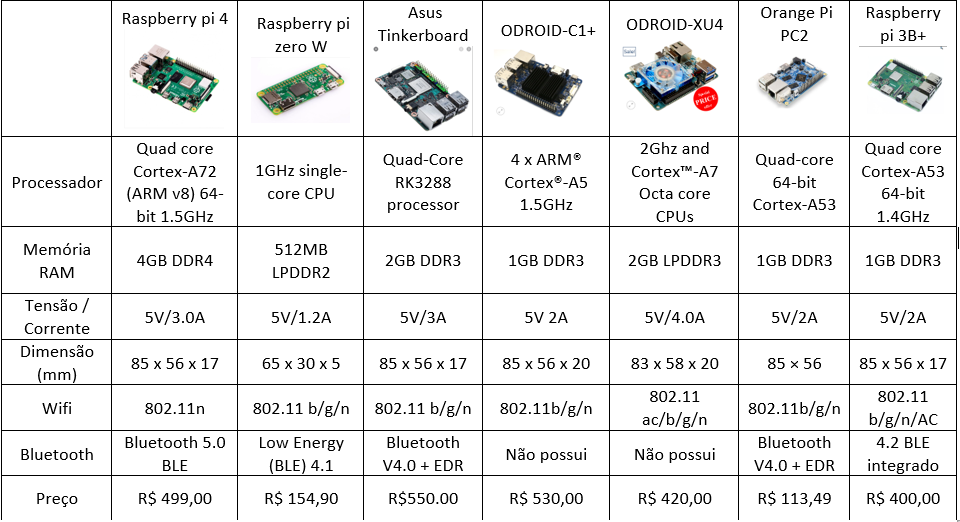
\includegraphics[scale=0.8]{figuras/SBCcomparacao.png}
  \caption{Tabela de comparação de \textit{single board computers}. Fonte : Autor } 
  \label{fig:comparacaoMicro}
\end{figure}

Após algumas reuniões, ficou decidido que se usaria a raspberry pi 3B+ no projeto. Porém, conforme as  \textit{sprints} foram passando, percebemos juntamente com o grupo de software que seria necessário mais capacidade de processamento para os algoritmos que seriam implementados. Um novo alinhamento geral foi feito e a escolha que melhor atenderia essa demanda de processamento seria o uso de uma Jetson Nano Developer Kit da Nvidia, mostrado na figura \ref{fig:Nvidea}. 

\begin{figure}[H]
  \centering
  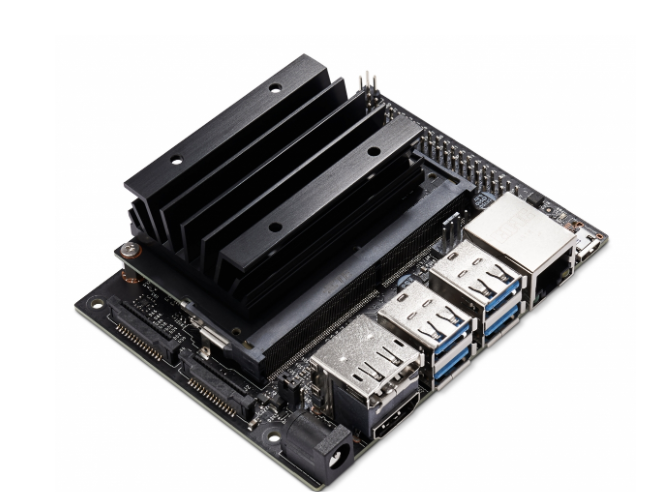
\includegraphics[scale=0.5]{figuras/NvideaPI2.png}
  \caption{Nvidea Jetson Nano Developer Kit. } 
  {\footnotesize Fonte : \cite{Nvidia_Nano} } 
  \label{fig:Nvidea}
\end{figure}

Apesar do detrimento causado no dimensionamento da bateria, essa placa foi escolhida devido a sua capacidade de processamento de algoritmos de  \textit{machine learning}, assim suprindo a demanda encaminhada pela equipe de \textit{software}.

Juntamente com a equipe de energia foi construído um diagrama de blocos das interligações dos componentes, o mesmo pode ser visto  na figura \ref{fig:CentraldeCOntrole}. Visto as colaborações necessárias entre os dois grupos com relação ao dimensionamento da bateria, por parte da energia, e o consumo de potência de cada componente por parte da eletrônica. 


\begin{figure}[H]
  \centering
  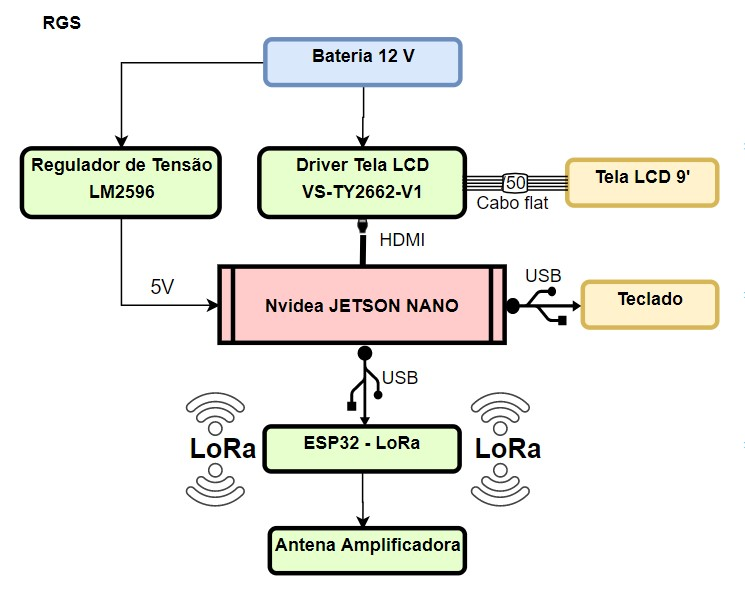
\includegraphics[scale=0.6]{figuras/Maleta_Diagrama.jpg}
  \caption{Diagrama Central de Controle. } 
  {\footnotesize Fonte : Autor } 
  \label{fig:CentraldeCOntrole}
\end{figure}

\subsection{Calibração}
Calibração é o processo de descobrir, experimentalmente, o Erro Sistemático (uma espécie de “desvio” constante) e a máxima Incerteza de Medição associada a um determinado instrumento. A forma mais comum de se realizar uma calibração é por meio da comparação direta do instrumento a ser calibrado com um instrumento de procedência conhecida, que é periodicamente avaliado com base em normas internacionais, conhecido como “Padrão” \cite{CALIBRACAO}.

Dentre os sensores utilizados na base de lançamento e no foguete, apenas as células de cargas da balança são transdutores necessários de calibração, os demais sensores já possuem calibração de fábrica, onde geralmente seus coeficientes de calibragem ficam armazenados em ROM.

Para calibrar a balança, após a montagem com as duas células de carga 50 Kg e o módulo conversor HX711, será rodado um programa de calibração no microcontrolador ESP32 LoRa. Através do programa deve ser encontrado o valor aferido do Fator de Calibração para  ser inserido no programa de medição da Balança com o conversor.

O programa de calibração fará uso da biblioteca \href{https://github.com/bogde/HX711}{HX711.h}, onde um objeto de peso conhecido deve ser lido pela balança, e a média dos valores retornados deve ser dividido pelo valor do peso real do objeto em KG, obtendo o fator de calibração, que deve ser inserido como parâmetro da função “scale.set\textunderscore scale()” importada da biblioteca mencionada. Com esse fator de calibração setado, obtém-se a medição do peso real do objeto \cite{CALIBRACAO_tutorial}.

A figura \ref{fig:Calibracao_balanca} apresenta o fluxograma do algoritmo de calibração dos sensores da balança.

\begin{figure}[H]
  \centering
  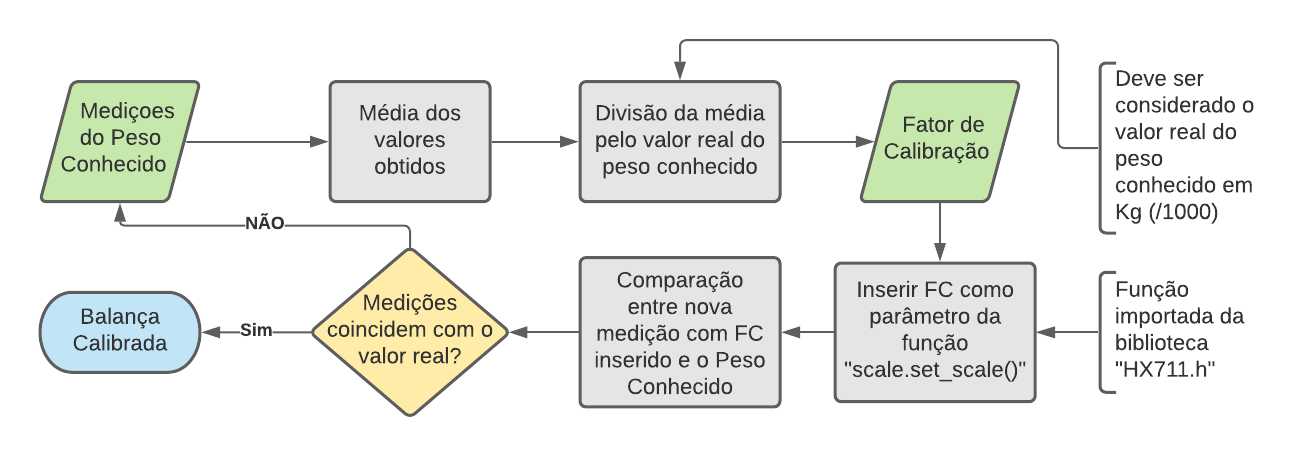
\includegraphics[scale=0.6]{figuras/Algoritmo de Calibração da Balança.png}
  \caption{Diagrama do algoritmo de calibração da balança } 
  {\footnotesize Fonte : Autor } 
  \label{fig:Calibracao_balanca}
\end{figure}


\subsection{Integrações}
\subsubsection{Diagrama de blocos do Abastecimento}
\par Apos reuniões com a equipe de estrutura e com a CRT, foram levantados os requisitos para o abastecimento do foguete de forma mais especifica. Foi criado um diagrama lógico para melhor entendimento do procedimento, figura \ref{fig:Abastecimento do fohuete}, e na sessão \ref{fig:sistema de alimentacao}. Assim, foi possível a equipe estrutural definir quais motores se enquadram para cada válvula do sistema.
\par É necessário um conjunto de 4 motores para a parte externa do foguete, um para a válvula 1 responsável por abrir o cilindro do combustível, um para a válvula 2 que é responsável por despressurizar a mangueira após a conclusão do abastecimento, dois para o desacoplamento do engate rápido, sendo que estes seriam acionados por um modulo de dois relés SRD‑05VDC‑SL‑C, por necessitarem se movimentarem somente em uma direção linear de desengate, diferentemente dos outros dois citados anteriormente, que necessitam se movimentarem nos dois sentidos (horário e antihorário, para abertura e fechamento das válvulas), fazendo-se necessário usar o modulo L298N, que é uma ponte H dupla.  
\par Já na parte interna do foguete, existem dois atuadores, que seriam acionados também de modo remoto: a válvula 4, que é uma válvula solenoide, responsável pelo controle da pressão do tanque do foguete, ou seja, ela fica abrindo e fechando a fim de estabilizar a pressão interna do foguete liberando gases internos durante o abastecimento; e a válvula 5, que é aberta na ignição, expulsando o óxido nitroso do tanque do foguete em direção à câmara de combustão. Ambas serão abertas em um só sentido; portanto, foi proposto usar um módulo de dois relés SRD‑05VDC‑SL‑C para seu acionamento pelo microcontrolador interno do foguete.
     


\begin{figure}[H]
  \centering
  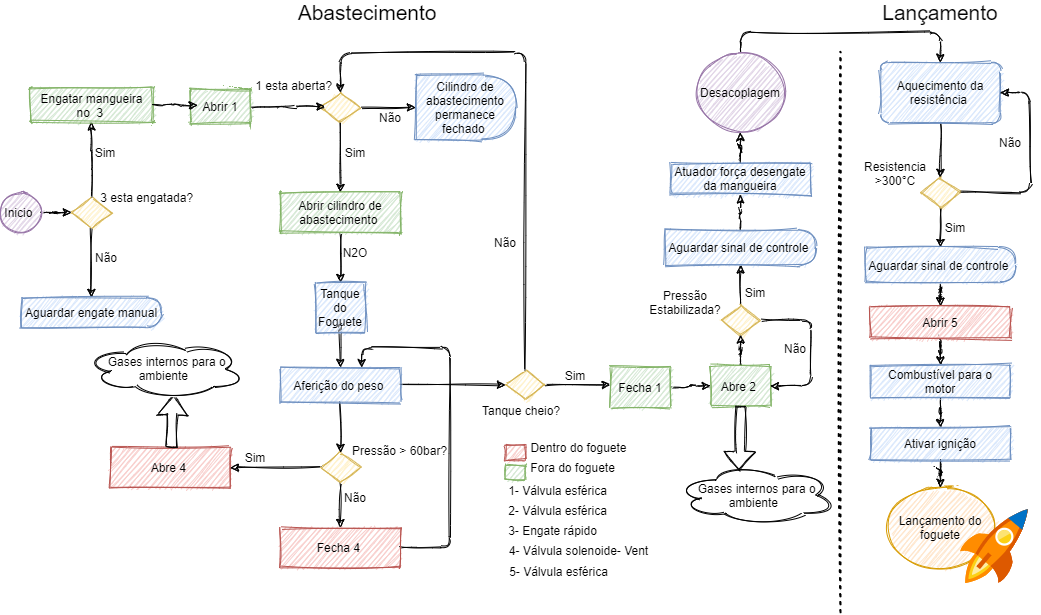
\includegraphics[scale=0.3]{figuras/abastecimento -Page-2 (2).png}
  \caption{ \href{https://drive.google.com/file/d/1EhMWyoD2Ml5I2vsLA0MbNOR8LxuCMmC5/view?usp=sharing}{ Diagrama logico do abastecimento foguete}. } 
  {\footnotesize Fonte : Autor } 
  \label{fig:Abastecimento do fohuete}
\end{figure}

\subsubsection{Acionamento eletrônico das válvulas externas}

As válvulas externas terão o seu acionamento controlado pelo microcontrolador ESP32 LoRa contido na base de lançamento do foguete, o qual também atua no controle da balança. Por meio dele serão enviados comandos de acionamento para fechar e abrir as válvulas externas durante o processo de abastecimento do foguete.

De acordo com informações obtidas do grupo de estrutura, serão necessários 3 adaptadores externos, sendo 2 válvulas esféricas que atuam no tanque de combustível e mangueira, e 1 atuador para desengate rápido, onde é necessário apenas o desengate remoto, pois o engate é manual. 

As válvulas esferas serão acionadas por meio de dois motores, um para cada válvula, onde o microcontrolador fará o seu acionamento por meio de uma Ponte H, enviando comandos para girar o motor em sentido horário ou anti-horário, ou seja, abrir ou fechar a válvula. A solução mecânica entre motores e válvulas é detalhado na estrutura.

De acordo com a estrutura, os motores usados para controle das válvulas esferas são do modelo Mabuchi 8d 12V. Esse motor é alimentado com 12V, com um consumo de corrente de 1,3A e torque de 9,12 N.m / 93 Kg. Para controle dos motores será necessário o uso de ponte H para realizar abertura e fechamento, controlando o sentido de rotação dos motores. 

A ponte H é um circuito que serve para variar o sentido da corrente em uma determinada carga, bem como controlar sua potência. A figura \ref{fig:PonteH_circuito} apresenta o circuito típico de uma ponte H.

\begin{figure}[H]
  \centering
  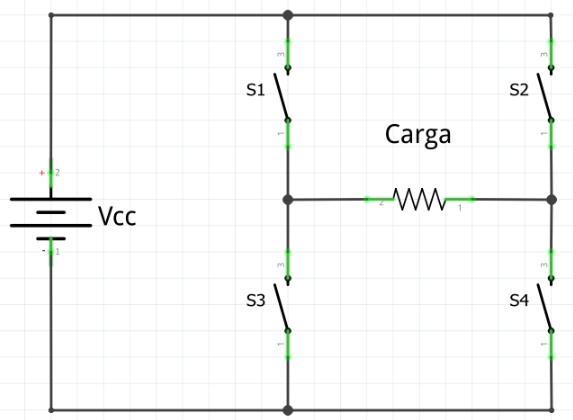
\includegraphics[scale=0.3]{figuras/ponteH_circuito.png}
  \caption{ Circuito típico de uma ponte H.} 
  {\footnotesize Fonte : \cite{PonteH_Teoria}} 
  \label{fig:PonteH_circuito}
\end{figure}

Com base nas especificações dos motores, foi escolhido o Driver Motor Ponte H L298n (cf. vide figura \ref{fig:PonteH_modulo}), para controle destes. Esse módulo possui tensão de operação de 4 a 35V, com corrente de operação máxima de 2A por canal (ou 4A máxima), tensão lógica de 5V, corrente lógica de 0 a 36mA e potência máxima de 25W \cite{PonteH_Datasheet}. O grande benefício desse módulo é que, com ele, é possível controlar dois motores ao mesmo tempo e, se necessário, controlar a velocidade deles, atuando no PWM do sinal enviado.

\begin{figure}[H]
  \centering
  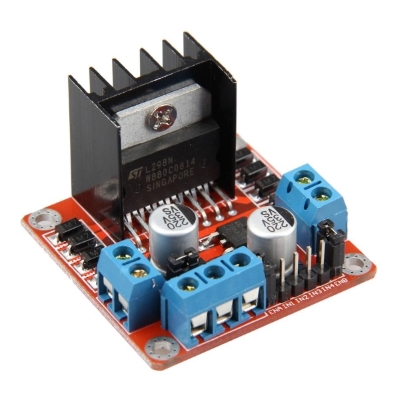
\includegraphics[scale=0.4]{figuras/ponteH_modulo.jpg}
  \caption{ Driver Motor Ponte H L298n.} 
  {\footnotesize Fonte : \cite{PonteH_mod}} 
  \label{fig:PonteH_modulo}
\end{figure}

Como o módulo da ponte H trabalha com tensão lógica de 5V, é necessário o uso de um conversor lógico de 3.3V (tensão lógica dos pinos da ESP32 LoRa) para 5V. Para tal, foi escolhido o Módulo Conversor Nível Lógico 5V/3.3V - Bidirecional (4 Canais), vide figura \ref{fig:CONV_LOGICO}. Esse conversor é capaz de elevar tensões de nível lógico de 3,3V para 5V, e isso de forma totalmente segura, possuindo 4 canais independentes que permitem a conversão de sinal. Entretanto, o conversor não é capaz de funcionar com sinais analógicos. A placa necessita de alimentação das duas voltagens (alta voltagem e baixa voltagem) com que seu sistema estiver trabalhando \cite{Conversor_logico}.

\begin{figure}[H]
  \centering
  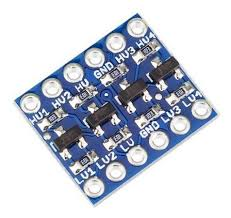
\includegraphics[scale=0.4]{figuras/conv_logico.jpeg}
  \caption{ Módulo Conversor Nível Lógico 5V/3.3V - Bidirecional (4 Canais)} 
  {\footnotesize Fonte : \cite{Conv_logico}} 
  \label{fig:CONV_LOGICO}
\end{figure}

Por fim, na parte externa ao foguete, tem-se o engate rápido, cuja solução mecânica não faz parte do escopo do projeto e sim da CRT. Todavia, apenas o acionamento eletrônico do seu desacoplamento do foguete faz parte do escopo da eletrônica, devido a necessidade de fazê-lo de maneira remota. 

Para tal, a solução adotada pela CRT é que o desacoplamento do engate seja feito com o auxílio de dois motores de vidro elétrico universal, modelo Mabuchi 8d 12v, o mesmo modelo utilizado para as válvulas esferas. O desacoplamento deve ocorrer quando os dois motores forem acionados em conjunto, onde cabos de aço presos no engate enrolaram no motor, puxando a mangueira para fora do engate.

Uma vez que os motores não precisarão inverter os sentidos de rotação, não é necessário o uso de ponte H, portanto, para realizar o acionamento dos motores, será utilizado um módulo  Módulo Relé 5V 2 Canais modelo SRD-05VDC-SL-C, vide figura \ref{fig:RELE_2CHANNEL}. Esse relé possui 2 canais, um para cada motor, possui tensão de operação de 5V, com um consumo de corrente típica de 15~20mA e possui capacidade na faixa de (30 VDC a 10A) ou (250VAC a 10A), o que atende a especificação dos motores Mabuchi \cite{rele_two}.

\begin{figure}[H]
  \centering
  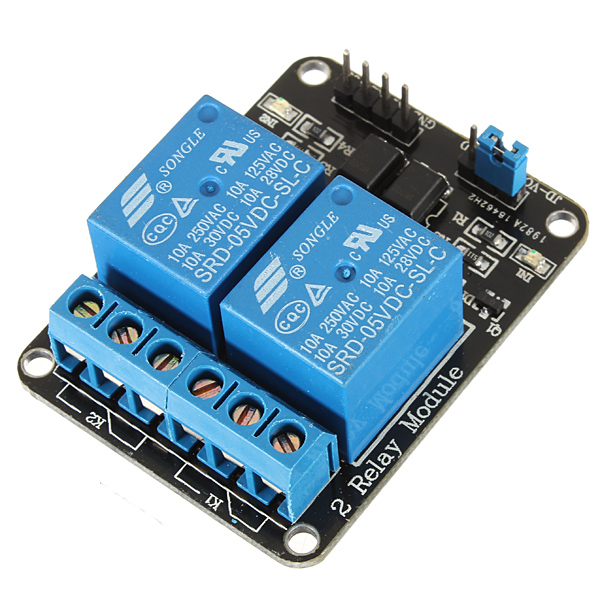
\includegraphics[scale=0.3]{figuras/RELE_2CHANNEL.jpg}
  \caption{ Módulo Relé 5V 2 Canais modelo SRD-05VDC-SL-C} 
  {\footnotesize Fonte : \cite{rele_photo}} 
  \label{fig:RELE_2CHANNEL}
\end{figure}

A conexão dos módulos atuadores das válvulas e do desengate no microcontrolador é estabelecido conforme esquema a seguir:

\begin{figure}[H]
  \centering
  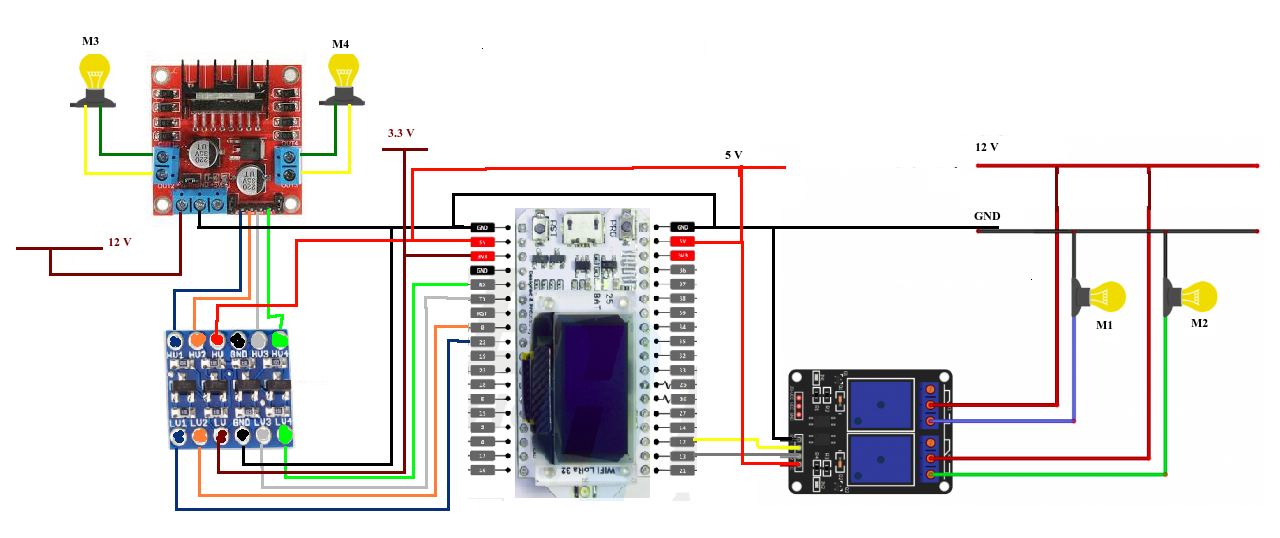
\includegraphics[scale=0.3]{figuras/BASE_VALVULAS.png}
  \caption{ Conexões entre atuadores externos e microcontrolador da base de lançamento. } 
  {\footnotesize Fonte : Autor}
  \label{fig:base_valvulas}
\end{figure}

onde, M1 e M2 são os dois motores do desengate remoto e M3 e M4 são os motores de abertura e fechamento das válvulas esferas do cilindro de combustível e mangueira, respectivamente.


\subsubsection{Acionamento eletrônico das válvulas internas}

\par As válvulas internas do foguete, serão controladas e acionadas pelo microcontrolador ESP32 LoRa presente no foguete, o qual também faz o controle dos sensores de pressão e temperatura e módulo GPS.
\par Uma vez que é necessário acionar com precisão a válvula 4, ou seja,  uma válvula solenoide, não é necessário o uso de ponte H. Portanto, para realizar o acionamento desta, será utilizado um relé que atende a necessidade de ficar acionando a válvula solenoide de tempo em tempos, e a outra válvula interna é do tipo esférica que será aberta somente uma vez também será acionado por relé,assim foi definido o uso do Módulo Relé 5V 2 Canais modelo SRD-05VDC-SL-C (cf. figura \ref{fig:RELE_2CHANNEL}), com as configurações supracitadas anteriormente. Esse relé possui 2 canais, um para a válvula solenoide e um para o motor da válvula 5 controlados pela ESP32-LoRa de dentro do foguete que mandará os sinais de controle para o modulo de relés e pode ser observado melhor no diagrama esquemático do circuito interno do foguete \ref{fig:Diagrama esquematico do circuito interno do foguete}.

\subsubsection{Comunicação hardware e software}

Visto que um dos maiores objetivos do projeto é a realização da telemetria com os dados vindos do foguete,este tópico tratará a maneira pela qual será realizada a comunicação entre o \textit{hardware} e a aplicação de \textit{software} e também como o dado trafegará em todo o sistema.

Para exemplificar de forma mais clara o caminho e os protocolos usados, a explicação será feita pro meio da figura \ref{fig:FLuxoDados}.

\begin{figure}[H]
  \centering
  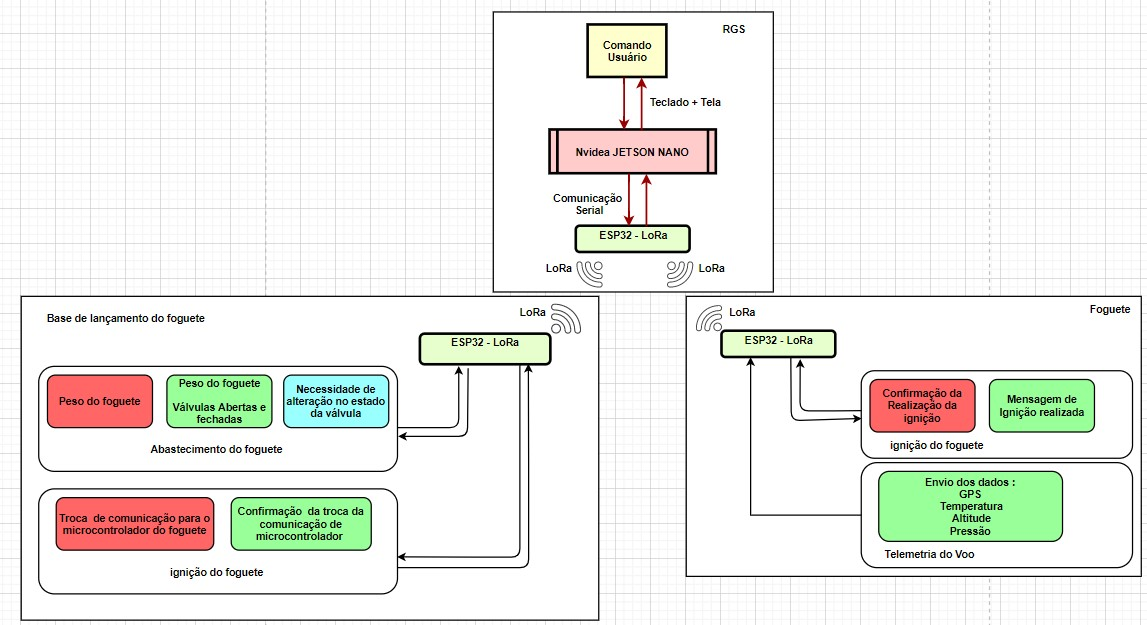
\includegraphics[scale=0.7]{figuras/Fluxo_dados.jpg}
  \caption{ Fluxo de dados} 
  {\footnotesize Fonte : Autor} 
  \label{fig:FLuxoDados}
\end{figure}

Todos os comandos são inseridos pelo usuário por meio do teclado, então o \textit{software} do sistema informa essas ações via comunicação serial para o microcontrolador da maleta, pois ambos estão conectados via USB. Esse primeiro passo está representado no topo da imagem anteriormente mostrada.

Assim que o comando chega neste primeiro microcontrolador, ele é transmitido para a base do foguete ou para o próprio foguete, dependendo se o lançamento está na faze do abastecimento ou da ignição.

Dependendo do tipo de comando, serão necessários dados informados pelo usuário (estes estão representados em vermelho no diagrama). Os blocos em verde são os dados enviados do \textit{hardware} para o \textit{software} desde que o processo tenha-se iniciado. Por fim, o bloco em azul representa as ações que podem ser realizadas durante a execução do comando.

Por exemplo, no caso do comando de abastecimento do foguete, quando requisitado pelo o usuário a realização desse processo, o \textit{hardware} requisitará o dado do bloco em vermelho. Quando o dado do bloco vermelho chegar, o hardware passará a transmitir, de forma contínua, os dados do bloco verde e, caso o usuário queira interferir na execução do processo, ele poderá tomar as ações do bloco azul. Então, para cada processo no lançamento do foguete, teremos essas requisições e envios dos dados de acordo com o diagrama.


\subsection{Diagramas e esquemáticos}

Com a definição da solução e dos componentes da base de lançamento, foi criado o esquemático do circuito integrado, com detalhamento de pinos, conexões e módulos utilizados. A figura \ref{fig:Diagrama esquematico do circuito interno da base de lancamento} apresenta o circuito integrado da base de lançamento, com os componentes da balança e os módulos dos atuadores externos, assim como bornes para os motores. Na figura \ref{fig:Diagrama esquematico do circuito interno do foguete}, encontra-se o diagrama esquemático, o detalhamento das conexões do sensoriamento interno do foguete, assim como a parte de controle das válvulas internas. Na figura \ref{fig:Diagrama esquematico do circuito interno da base de lancamento}, por sua vez, tem-se o esquemático com as conexões na base central de comando entre a ESP32 WifiLora e a Jetson e outros periféricos. Os esquemáticos foram feitos utilizando as ferramentas do \textit{software} EasyEDA ,assim como o projeto de suas PCIs.

\begin{figure}[H]
  \centering
  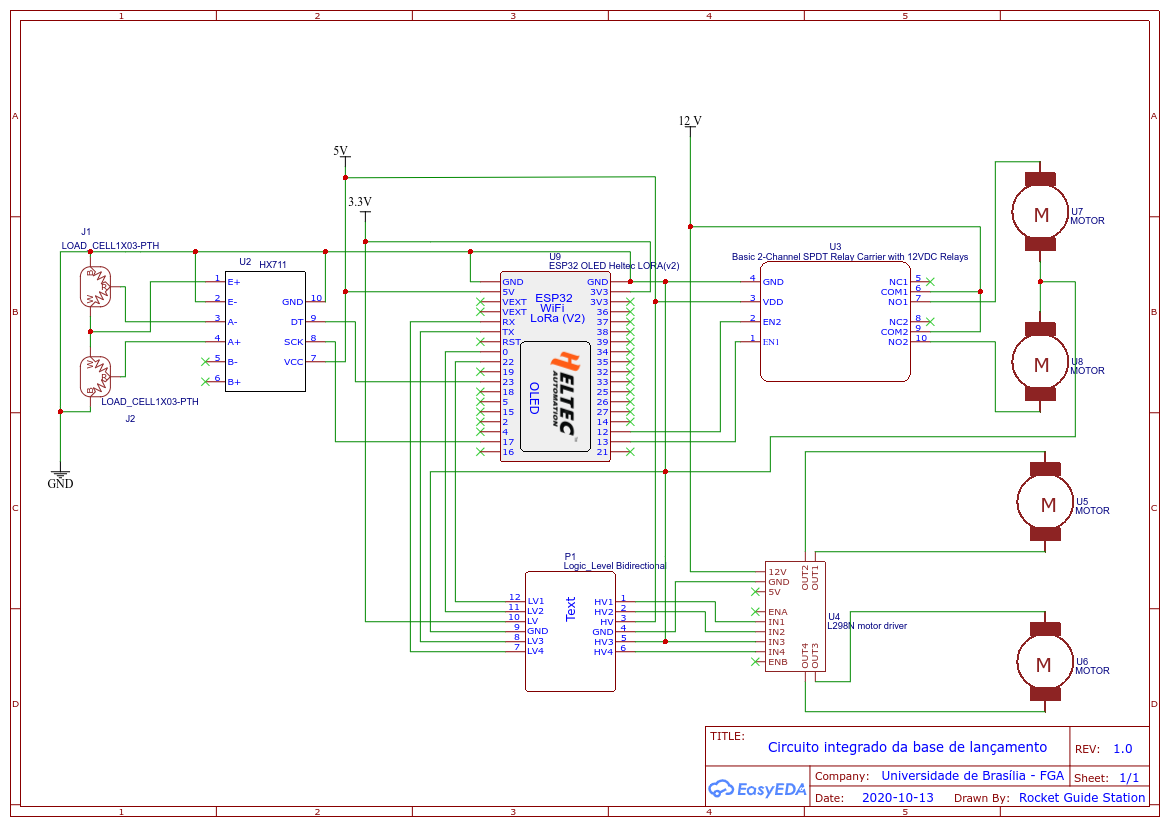
\includegraphics[scale=0.4]{figuras/Schematic_Base_Lancamento.png}
  \caption{Diagrama esquemático do circuito interno da base de lançamento.} 
  {\footnotesize Fonte : Autor } 
  \label{fig:Diagrama esquematico do circuito interno da base de lancamento}
\end{figure}

\begin{figure}[H]
  \centering
  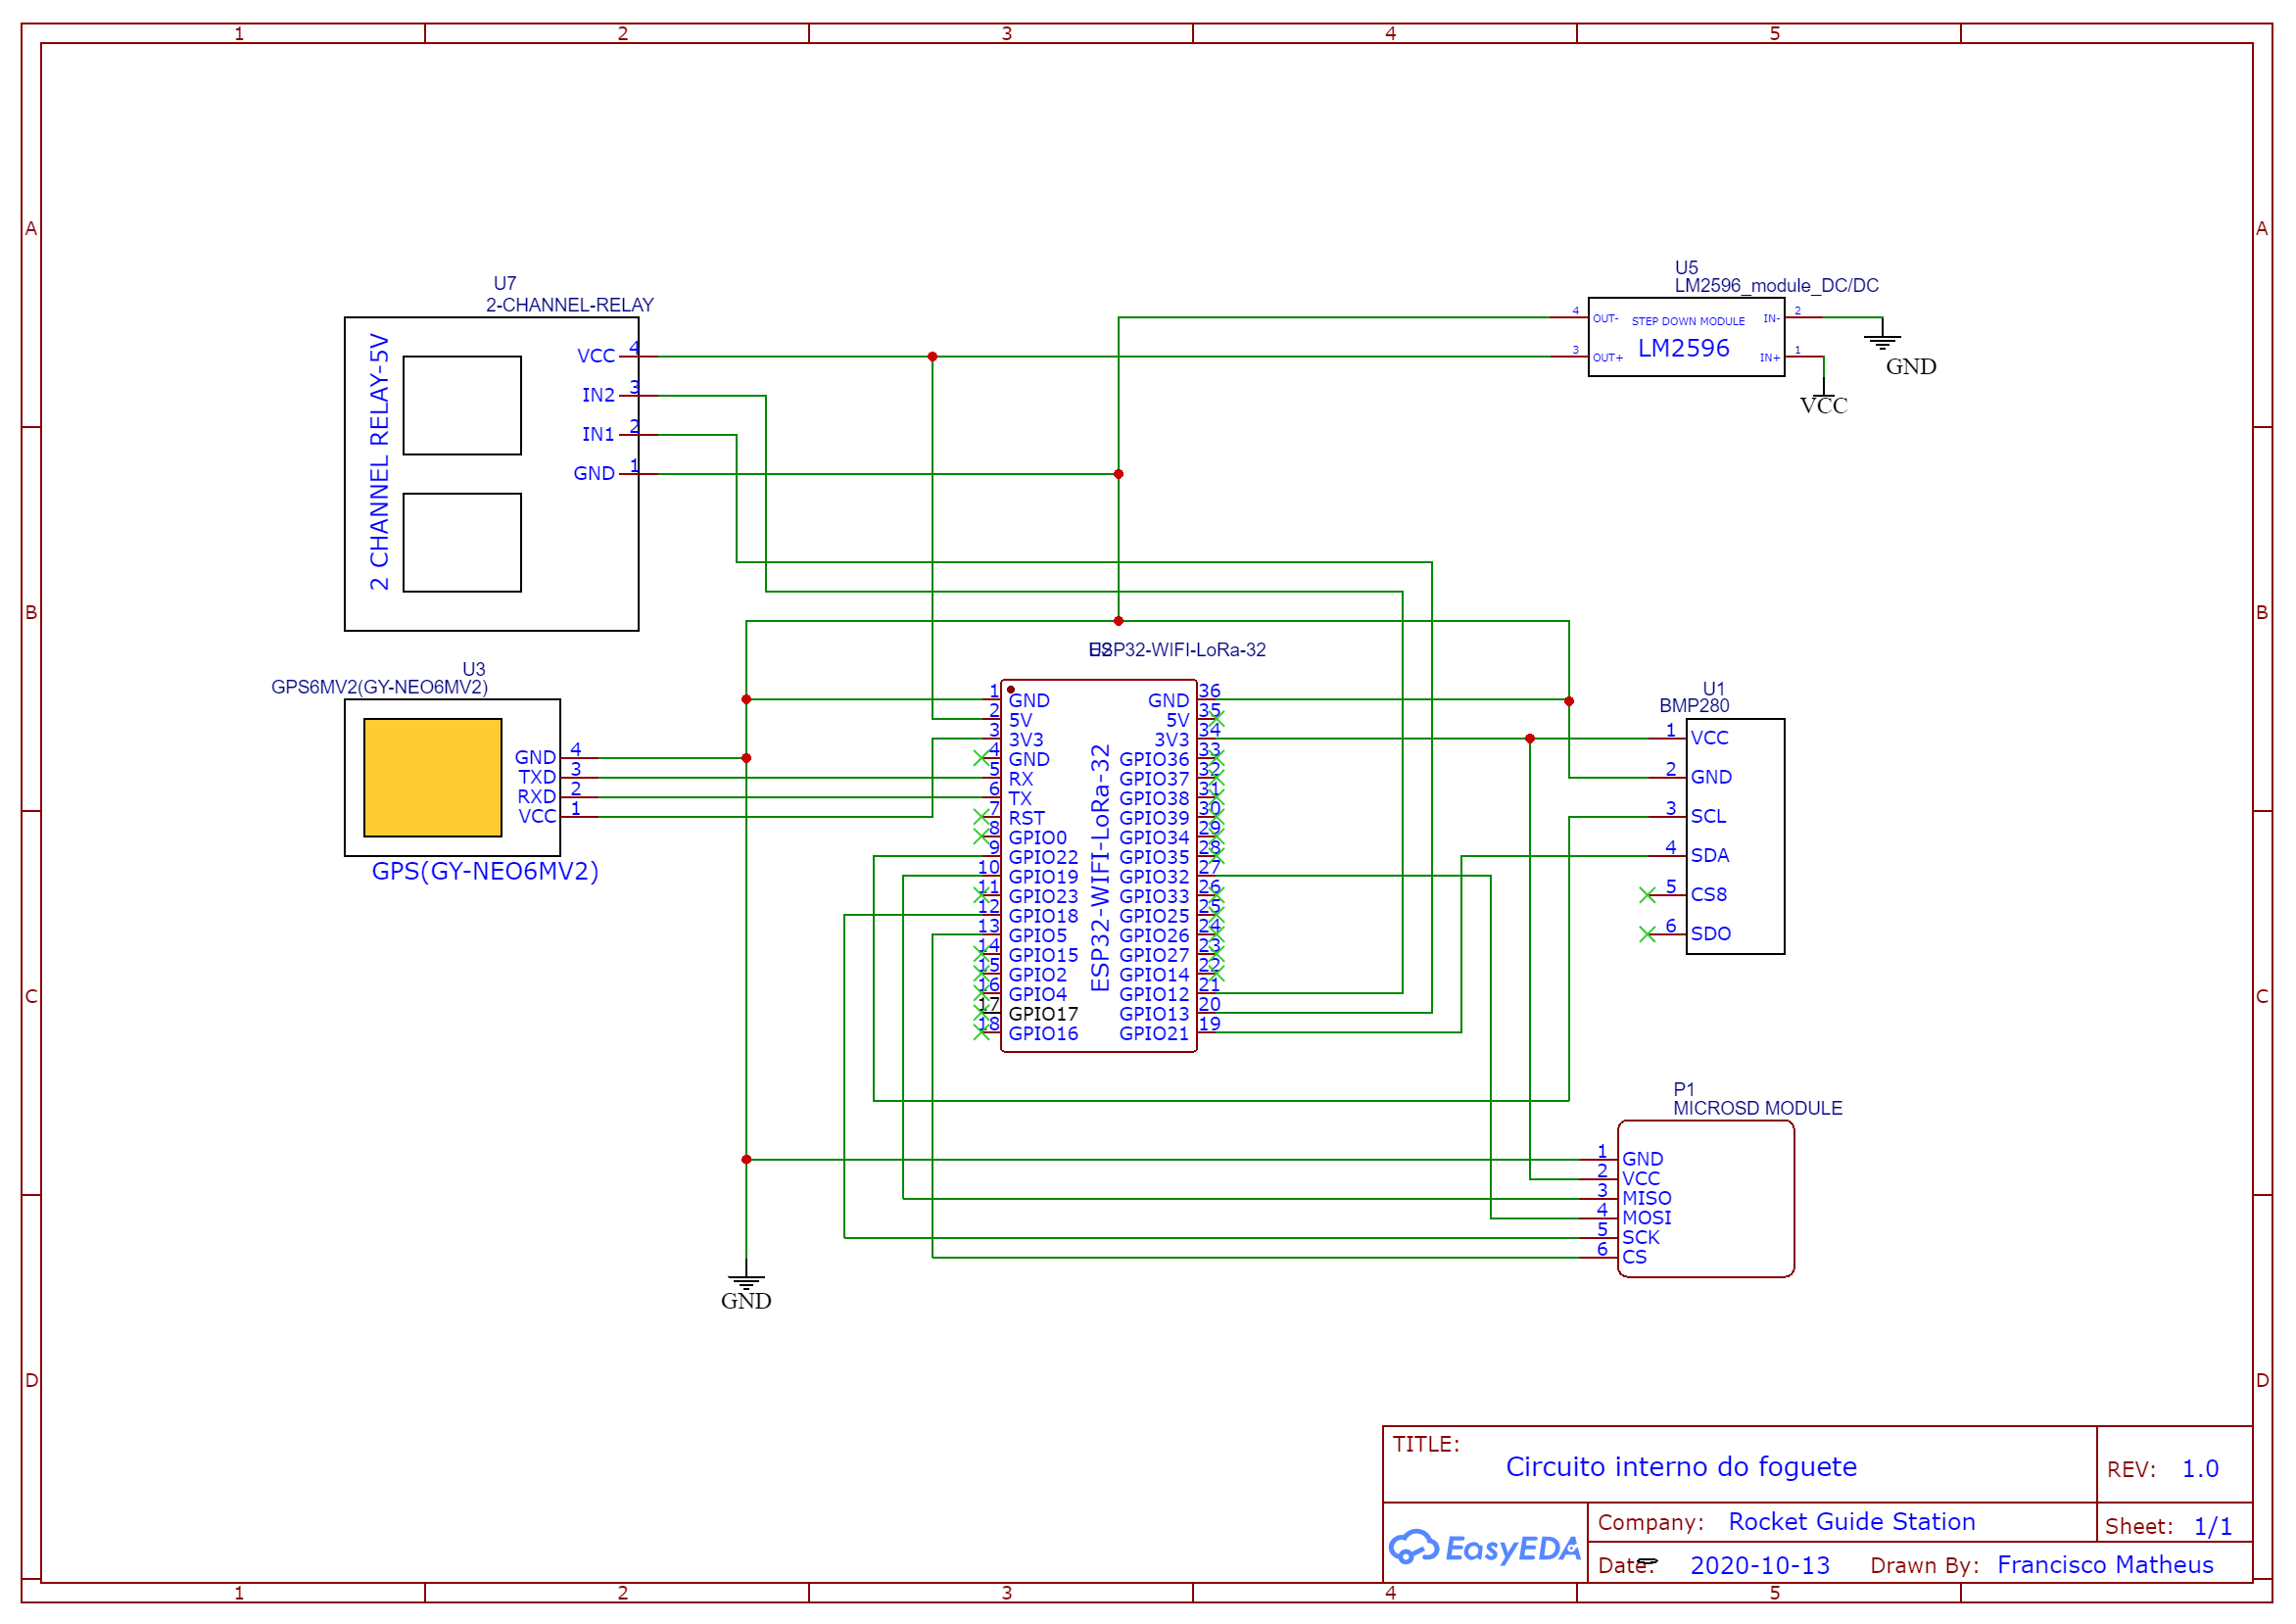
\includegraphics[scale=0.18]{figuras/Esquematico circuito interno ao foguete.png}
  \caption{Diagrama esquemático do circuito interno do foguete. } 
  {\footnotesize Fonte : Autor } 
  \label{fig:Diagrama esquematico do circuito interno do foguete}
\end{figure}

\begin{figure}[H]
  \centering
  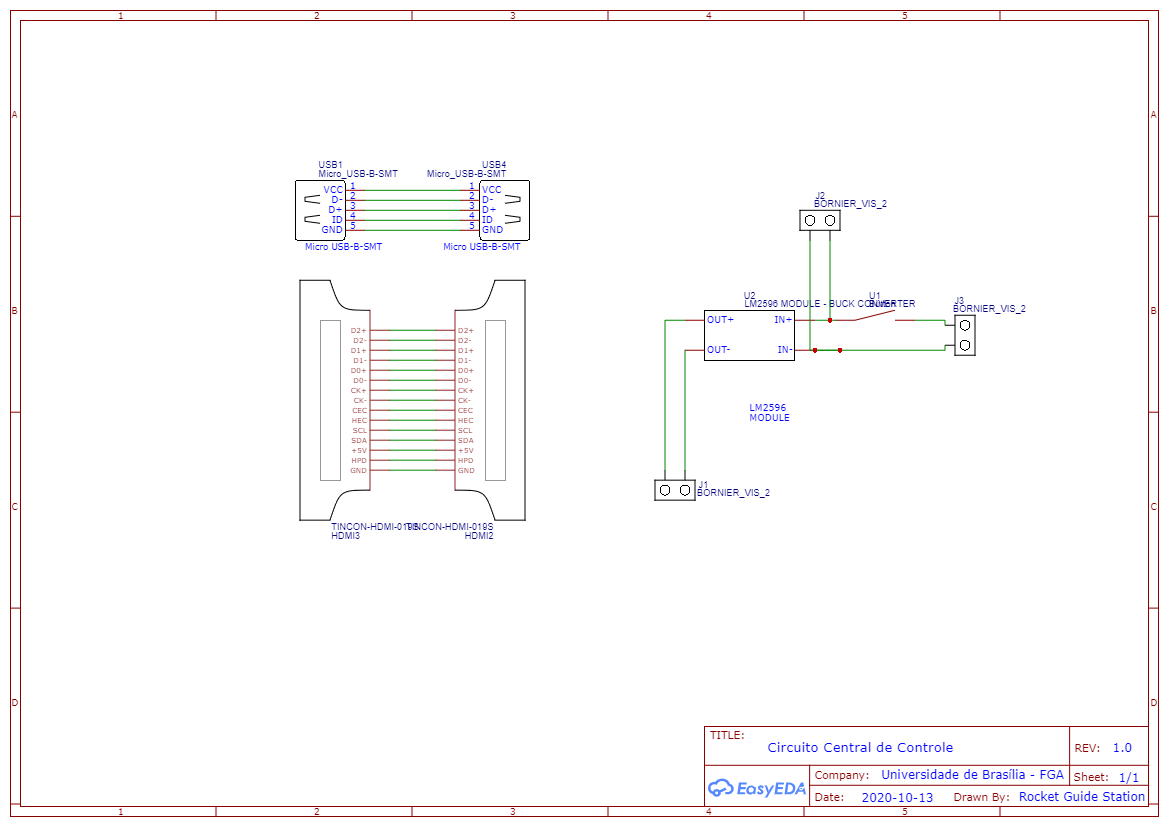
\includegraphics[scale=0.35]{figuras/Schematic_Maleta.png}
  \caption{Diagrama esquemático do circuito da central de controle do usuário.} 
  {\footnotesize Fonte : Autor } 
  \label{fig:Diagrama esquemático do circuito da central de controle do usuário}
\end{figure}

\subsection{Placa de circuito impresso}

\par Para melhor funcionamento  e durabilidade do circuito, é necessária a criação do desenho de placa de circuito impresso, conhecido como PCI, que é gerido por regras que visam garantir a qualidade do funcionamento do circuito, até visando a disposição dos componentes para melhor acomodação mecânica e eletromagnética, a fim de evitar interferências no circuito.
\par Basicamente, é constituída por uma base de um material isolante, geralmente fenolite ou fibra de vidro, revestida por uma fina camada de cobre na sua superfície, onde ocorre as ligações entres os componente eletrônicos que podem ser do tipo PTH ou SMD\cite{pci}. 

\par As placas utilizadas nesse projeto serão feitas de modo a acomodar componentes do tipo PTH, ou seja, componentes que serão inseridos na placa através de um furo denominado de pads, sendo necessário uma acurácia para não errar no distanciamento dos furos, evitando assim mal posicionamento dos componentes eletrônicos.
\par Outro levantamento importante que é necessário fazer no projeto de uma PCI é a largura das trilha, que são responsáveis pelas conexões elétricas entre os componentes, a qual é determinada pela corrente que irá passar pela trilha e pela espessura da trilha de cobre \cite{ TecnicasdeProjetosPCI}.

\subsubsection{Circuito interno do foguete}
\par Na figura \ref{fig:Diagrama esquematico do circuito interno do foguete}, está representado o circuito interno do foguete. Assim, na figura \ref{fig:PCIFOGUETE}, encontra-se o  projeto mecânico da placa de circuito impresso com as dimensões para sua fabricação. Foram adicionados cinco buracos na PCI no intuito de facilitar sua fixação dentro do foguete com parafusos de diâmetro de 5mm. Na figura \ref{fig:PCB_FOGUETE}, por sua vez, é apresentado o modelo 3D da PCI com com o sistema de alimentação à esquerda da placa, separado dos outros componentes a fim de evitar interferência eletromagnética no restante da placa. Foi adicionado a essa placa esse sistema para garantir a tensão adequada para os componentes. 
\par A placa a ser produzida possui espessura padrão de 1,6mm, com tolerância nominal de $\frac{+}{-}$ 0,13mm. Nessa PCB específica, são utilizadas duas camadas de cobre para as trilhas; portanto, serão feitas trilhas tanto na \textit{Top Layer} quanto na \textit{Bottom Layer}, ou seja, \textit{multilayer}, garantindo uma melhor distribuição das trilhas. Por ser um módulo que vai dentro do foguete, inicialmente foi pensado em usar componentes do tipo PTH e a plaquinha de desenvolvimento da ESP32Lora, da Heltec, pois não são feitos muitos lançamentos. A ideia é utilizar primeiramente uma PCB nesse formato para testes e melhorias no projeto, antes de confeccionar uma placa mais enxuta com componentes SMD. 
\par Para essa versão inicial das placas de circuito impresso, seriam feitas de fenolite (FR2), que é um material mais barato para a confecção e quando tiver os componentes testados será feito em material de vibra de vidro(FR4)\cite{CONCEITOpci}.

\begin{figure}[H]
  \centering
  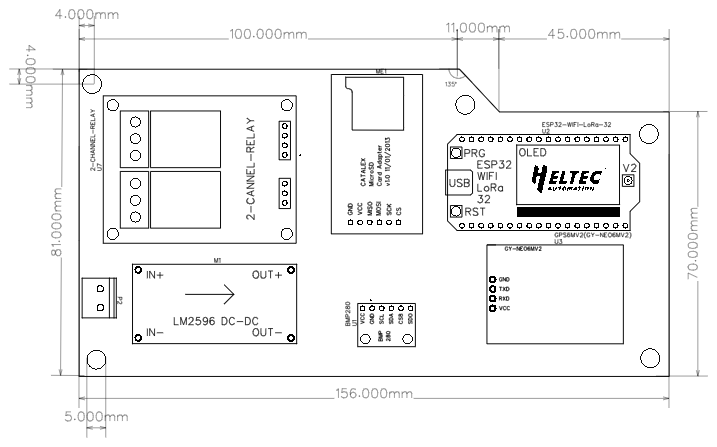
\includegraphics[scale=0.5]{figuras/PCB-FOGUETE COTAGEM.png}
  \caption{ Dimensões da PCI do circuito interno do foguete. } 
  {\footnotesize Fonte : Autor } 
  \label{fig:PCIFOGUETE}
\end{figure}

\begin{figure}[H]
  \centering
  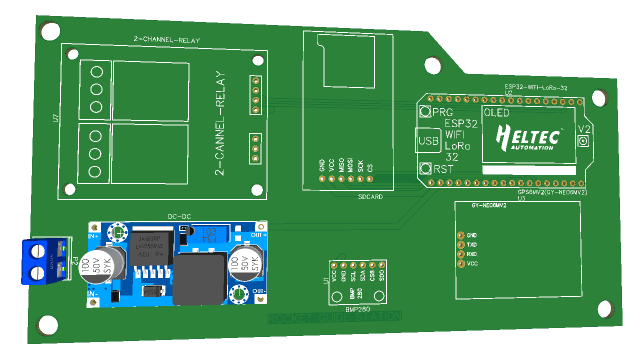
\includegraphics[scale=0.4]{figuras/PCI-FOGUETE TV2.png}.
    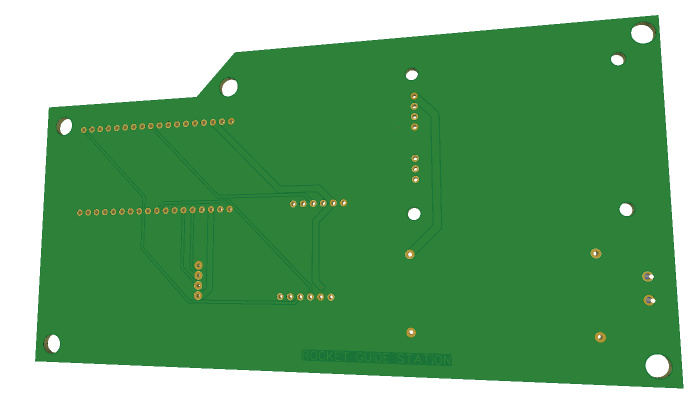
\includegraphics[scale=0.4]{figuras/PCI-FOGUETE BV2.png}
  \caption{PCI do circuito interno do foguete. } 
  {\footnotesize Fonte : Autor } 
  \label{fig:PCB_FOGUETE}
\end{figure}





\subsubsection{Circuito na base de lançamento}

Objetivando reduzir o número de fios e cabos utilizados no circuito da base de lançamento, assim como obter a menor ocupação de volume de circuitaria e componentes, foi criado o modelo de PCI com base no circuito integrado citado na figura \ref{fig:Diagrama esquematico do circuito interno da base de lancamento}. Foi optado o modelo \textit{Bottom Layer} para as trilhas da PCI, ou seja, contém apenas uma camada de cobre.

A figura \ref{fig:PCB_BASE_LANCAMENTO_DES} mostra o desenho da PCI, junto com suas cotas de dimensões definidas, que foram de 88mm x 109mm. Os buracos nos cantos da PCB, com diâmetro de 4mm e distâncias das bordas de 3mm, servem pra fixação da placa na estrutura da base.

\begin{figure}[H]
  \centering
  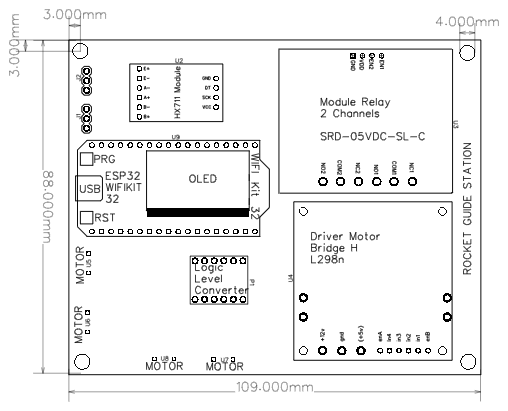
\includegraphics[scale=0.5]{figuras/PCB_Base_Lancamento_Desenho.png}
  \caption{ Dimensões da PCI do circuito interno da base de lançamento. } 
  {\footnotesize Fonte : Autor } 
  \label{fig:PCB_BASE_LANCAMENTO_DES}
\end{figure}

A figura \ref{fig:PCB_BASE_LANCAMENTO} apresenta a visão frontal da PCI, onde é possível visualizar a posição dos componentes, tais como encaixes dos pinos e os bornes dispostos nas extremidades, e a visão traseira da PCI, onde se encontra a camada de fundo (\textit{Bottom Layer}), com as trilhas do circuito.

\begin{figure}[H]
  \centering
  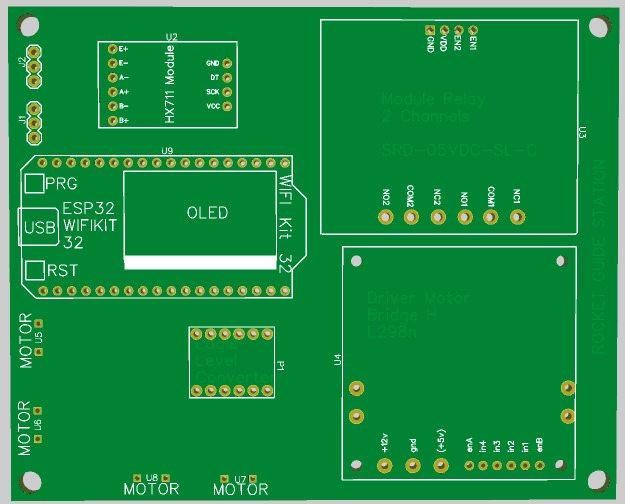
\includegraphics[scale=0.3]{figuras/PCB_Base_Lancamento_Front.jpeg}
    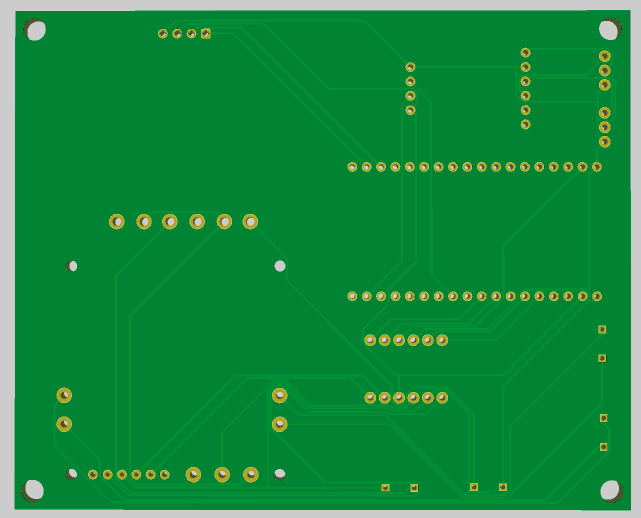
\includegraphics[scale=0.3]{figuras/PCB_Base_Lancamento_Back.jpeg}
  \caption{PCI do circuito interno da base de lançamento } 
  {\footnotesize Fonte : Autor } 
  \label{fig:PCB_BASE_LANCAMENTO}
\end{figure}

\subsubsection{Circuito na base de controle central}

A ideia dessa PCI é reduzir o número de cabos utilizados dentro da maleta do usuário.
De acordo com o espaço e a disposição dos componentes mostrado na figura  \ref{fig:Disposicao dos Componentes} e na figura \ref{fig:PCB_controle} pensou-se em fazer uma placa de modo que os módulos sejam encaixados nas laterais da PCI. Para isso foi verificado todos desenhos técnicos dos componentes, mapeando então os conectores  por meio dessas medidas fornecidas pelo fabricante. Os conectores precisarão ser do tipo macho para que o encaixe seja realizado. Isso traz vantagens: caso algum módulo sofra dano, bastará  desconectá-lo e realizar a troca.

\begin{figure}[H]
  \centering
  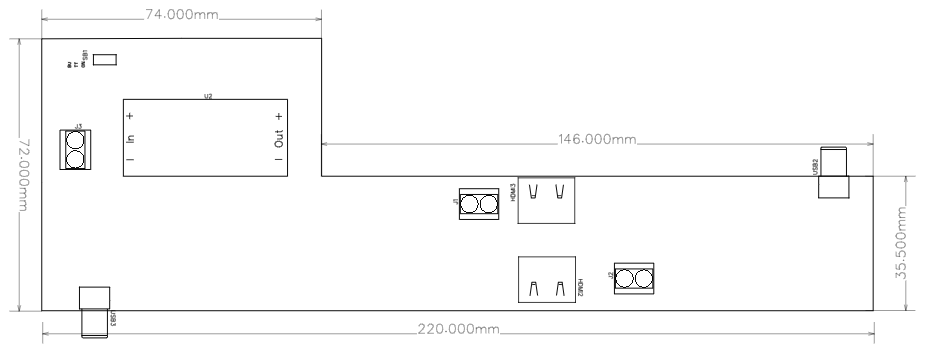
\includegraphics[scale=0.5]{figuras/PCB_Maleta.png}
  \caption{ Dimensões da PCI do circuito da central de controle.} 
  {\footnotesize Fonte : Autor } 
  \label{fig:PCIMaleta}
\end{figure}

\begin{figure}[H]
  \centering
  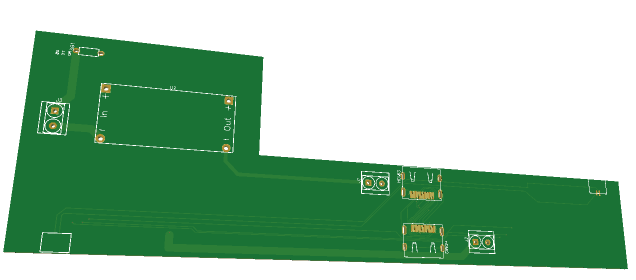
\includegraphics[scale=0.4]{figuras/pcicontrole-top.png}
    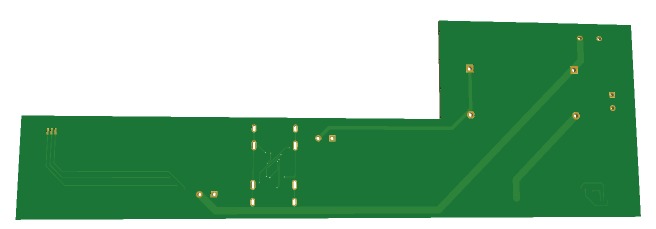
\includegraphics[scale=0.4]{figuras/pcicontrole-bo.png}
  \caption{PCI do circuito interno do foguete. } 
  {\footnotesize Fonte : Autor } 
  \label{fig:PCB_controle}
\end{figure}
